

\documentclass[11pt,a4paper,oneside]{report}

% Lingua, codifica e impaginazione
\usepackage[italian]{babel}
\usepackage[T1]{fontenc}
\usepackage[utf8]{inputenc}
\usepackage{lmodern}
\usepackage[a4paper,margin=2.8cm]{geometry}
\usepackage{microtype}

% Matematica, codice e figure
\usepackage{amsmath,amssymb}
\usepackage{graphicx}
\usepackage{booktabs}
\usepackage{siunitx}
\usepackage{xcolor}
\usepackage{listings}
\usepackage{float}

% Collegamenti e indice
\usepackage[hidelinks]{hyperref}
\usepackage{bookmark}

% Ambienti per definizioni e osservazioni
\usepackage{amsthm}
\newtheorem{definizione}{Definizione}[chapter]
\newtheorem{teorema}{Teorema}[chapter]
\newtheorem{esempio}{Esempio}[chapter]
\theoremstyle{remark}
\newtheorem*{osservazione}{Osservazione}

% Stile del codice
\lstset{
	basicstyle=\ttfamily\small,
	frame=single,
	breaklines=true,
	columns=fullflexible,
	numbers=left,
	numberstyle=\tiny\color{gray},
	keywordstyle=\color{blue!70!black},
	commentstyle=\color{green!40!black},
	showstringspaces=false,
	literate=
		{à}{{\`a}}1
		{è}{{\`e}}1
		{é}{{\'e}}1
		{ì}{{\`i}}1
		{ò}{{\`o}}1
		{ù}{{\`u}}1
}

\usepackage[T1]{fontenc}
\usepackage[utf8]{inputenc}
\usepackage[italian]{babel}

\theoremstyle{definition}
\newtheorem{definition}{Definizione}[chapter]
\newtheorem{example}{Esempio}[chapter]

\theoremstyle{remark}
\newtheorem{remark}{Osservazione}[chapter]


\begin{document}

\title{Data Science e Tecnologie per le Basi di Dati}
\author{Antonio Villella}
\date{Anno accademico 2026--2027}

\maketitle



\tableofcontents



\chapter*{Introduzione al Corso e Modalità d'Esame}

\section*{Descrizione dell'Insegnamento}
L'insegnamento di Data Science e Tecnologie per le Basi di Dati è un corso obbligatorio per la Laurea Magistrale in Ingegneria Informatica. L'obiettivo principale del corso è descrivere gli aspetti fondamentali della tecnologia dei sistemi per la gestione delle basi di dati (DBMS) e le metodologie di gestione delle basi di dati destinate all'analisi (comunemente denominate data warehouse). 

Questi sistemi si caratterizzano per la necessità di gestire enormi volumi di dati. Nel corso vengono esplorate sia le tecniche di analisi tradizionali, come l'analisi OLAP (On Line Analytical Processing), sia tecniche di analisi più complesse basate sul data mining.

\section*{Programma e Argomenti Trattati}
Il programma del corso si articola in diverse macro-aree fondamentali per la gestione e l'analisi dei dati:
\begin{itemize}
    \item \textbf{Caratteristiche tecnologiche dei DBMS:} vengono studiati la gestione dell'accesso concorrente ai dati, l'affidabilità del sistema, le strutture del livello fisico e l'ottimizzazione dell'accesso ai dati.
    \item \textbf{Basi di dati NoSQL:} introduzione al modello dei dati e ai linguaggi di interrogazione di sistemi non relazionali, con particolare riferimento a MongoDB ed Elastic.
    \item \textbf{Basi di dati distribuite:} studio dell'architettura dei sistemi distribuiti e delle relative tecniche di gestione della replicazione.
    \item \textbf{Data warehouse (DW):} analisi dell'architettura e delle metodologie di progettazione concettuale, logica e fisica. Vengono inoltre trattate la preparazione dei dati e la formulazione di interrogazioni OLAP tramite il linguaggio SQL.
    \item \textbf{Data science e Machine learning:} panoramica sul processo di data science e approfondimento dei principali algoritmi di apprendimento automatico per la classificazione, il clustering e l'estrazione di regole di associazione.
\end{itemize}

\section*{Struttura e Regole dell'Esame}
L'esame si compone di una prova scritta obbligatoria e della valutazione di eventuali homework assegnati durante il semestre (elaborato progettuale individuale). Gli homework sono facoltativi, ma fortemente consigliati. A discrezione del docente, potrebbe essere richiesta una prova integrativa a conferma del voto ottenuto.

\subsection*{La Prova Scritta}
La prova scritta si svolge in aula tramite PC, utilizzando la piattaforma di ateneo, e ha una durata complessiva di 100 minuti. Durante lo svolgimento non è permesso l'utilizzo di libri, appunti o dispositivi elettronici di alcun tipo.

Il test è composto da domande a risposta aperta e chiusa, oltre a esercizi pratici di progettazione. Le regole di valutazione delle domande prevedono che le risposte errate ai quesiti a risposta chiusa comportino una penalizzazione, mentre le risposte omesse valgano zero.

L*a struttura tipica della prova scritta è la seguente:
\begin{itemize}
    \item \textbf{Domande teoriche (6-8 quesiti):} vertono sui concetti principali del corso, quali aspetti tecnologici dei DBMS, basi di dati distribuite, preparazione dei dati e algoritmi di analisi (massimo 8 punti).
    \item \textbf{Progettazione fisica (1-3 esercizi):} esercizi sulla creazione di strutture fisiche per basi di dati (massimo 3 punti).
    \item \textbf{Progettazione Data Warehouse (1-2 esercizi):} modellazione di un DW (massimo 5 punti).
    \item \textbf{Preparazione dei dati (1 esercizio):} operazioni di data preparation per data warehouse in linguaggio SQL (massimo 5 punti).
    \item \textbf{Interrogazioni OLAP (3 esercizi):} scrittura di istruzioni SQL per l'accesso e l'analisi dei dati di un data warehouse (massimo 11 punti).
\end{itemize}

\subsection*{Homework e Valutazione Finale}
Durante il corso verranno proposti quattro homework individuali. Questi lavori sono mirati a sviluppare il pensiero critico e le capacità di problem solving sugli argomenti trattati a lezione. 

Per quanto riguarda il calcolo del voto finale:
\begin{itemize}
    \item Gli homework possono conferire un massimo di 2 punti aggiuntivi.
    \item Le relazioni degli homework vengono prese in considerazione per il voto finale esclusivamente se la valutazione della prova scritta è pari o superiore a 18/30.
    \item La lode viene assegnata nel caso in cui il punteggio complessivo superi il 31/30.
\end{itemize}
\chapter{Data Science e The Big Data Challenge}

\section{Introduzione ai Big Data}
Il concetto di \textbf{Big Data} ha molteplici definizioni, essendo un termine che si è evoluto rapidamente nel corso degli anni (spesso accompagnato da un forte \textit{hype} mediatico, come ironicamente illustrato in celebri vignette a tema). Tuttavia, da un punto di vista accademico e tecnologico, possiamo adottare la seguente definizione formale:

\begin{definition}[Big Data]
I Big Data sono dati la cui \textbf{scala, diversità e complessità} richiedono nuove architetture, tecniche, algoritmi e strumenti di analisi (\textit{analytics}) per poterli gestire ed estrarne valore e conoscenza nascosta.
\end{definition}

% FIGURA DA INSERIRE QUI
% Fonte: Slide 1
% Descrizione: Striscia a fumetti di Dilbert sull'hype dei Big Data.
\begin{figure}[H]
    \centering
    % \includegraphics[width=0.7\textwidth]{dilbert_big_data}
    \caption{L'hype mediatico attorno al concetto di Big Data.}
    \label{fig:dilbert_bigdata}
\end{figure}

\section{Le Sfide dei Big Data}
L'avvento dei Big Data introduce delle sfide significative che non possono essere affrontate con i sistemi tradizionali. Queste sfide si dividono in due macro-categorie:

\subsection{Tecnologia e infrastruttura}
La gestione di moli di dati così imponenti richiede nuovi paradigmi di programmazione e nuove architetture hardware/software. Il principio fondamentale che guida queste nuove tecnologie è:
\begin{center}
    \textit{"Transfer the processing power to the data"} \\
    (Trasferire la potenza di calcolo verso i dati)
\end{center}
Invece di spostare enormi quantità di dati verso i server di calcolo (operazione lenta e costosa in termini di rete), si spostano gli algoritmi e il calcolo direttamente sui nodi dove i dati sono immagazzinati. L'ecosistema di riferimento per questo paradigma è \textbf{Apache Hadoop} e \textbf{Apache Spark}.

% FIGURA DA INSERIRE QUI
% Fonte: Slide 4
% Descrizione: Logo dell'elefantino di Apache Hadoop.
\begin{figure}[H]
    \centering
    % \includegraphics[width=0.3\textwidth]{hadoop_elephant}
    \caption{L'ecosistema Apache Hadoop è una delle tecnologie fondanti per gestire le infrastrutture Big Data.}
    \label{fig:hadoop_elephant}
\end{figure}

\subsection{Gestione e analisi dei dati}
Oltre all'infrastruttura, c'è una nuova e forte enfasi sul "dato" in sé. Raccogliere i dati non basta: è necessario analizzarli per estrarne valore. Questa esigenza ha dato vita a una disciplina specifica: la \textbf{Data Science}.

\section{Data Science}
La Data Science è la disciplina che si occupa di \textit{"estrarre significato da grandissime quantità di dati"}. 
È un campo fortemente multidisciplinare che unisce statistica, machine learning, data mining, visualizzazione dei dati e gestione dei database.

\begin{remark}
Il termine \textit{"Data Scientist"} è stato coniato originariamente da D.J. Patil (ex Chief Data Scientist degli Stati Uniti), contribuendo a definire una nuova figura professionale fondamentale nel panorama tecnologico moderno.
\end{remark}

% FIGURA DA INSERIRE QUI
% Fonte: Slide 5
% Descrizione: Mappa concettuale che mostra le varie discipline che compongono la Data Science (Statistic, Machine Learning, Data Mining, ecc.).
\begin{figure}[H]
    \centering
    % \includegraphics[width=0.6\textwidth]{data_science_mindmap}
    \caption{La natura multidisciplinare della Data Science.}
    \label{fig:ds_mindmap}
\end{figure}

\section{Il Processo di Data Science (KDD)}
Il processo di estrazione della conoscenza dai dati è formalmente noto come \textbf{KDD} (\textit{Knowledge Discovery in Databases}). 

Il flusso di lavoro della Data Science si articola in una macro-pipeline composta da quattro fasi principali, disposte in sequenza logica:
\begin{enumerate}
    \item \textbf{Generation} (Generazione del dato)
    \item \textbf{Acquisition} (Acquisizione)
    \item \textbf{Storage} (Memorizzazione)
    \item \textbf{Analysis} (Analisi)
\end{enumerate}

% FIGURA DA INSERIRE QUI
% Fonte: Slide 6
% Descrizione: I due schemi del processo KDD. Da un lato il processo lineare (Data -> Preprocessing -> Data Mining -> Knowledge), dall'altro il ciclo di feedback continuo con il mondo reale (Real World -> Raw Data -> Model -> Data Product -> Real World).
\begin{figure}[H]
    \centering
    % \includegraphics[width=0.9\textwidth]{kdd_process}
    \caption{Rappresentazione del processo KDD (Knowledge Discovery in Databases) e del ciclo di vita di un Data Product.}
    \label{fig:kdd_process}
\end{figure}

\subsection{Fase 1: Generazione dei dati (Generation)}
La prima fase del processo KDD riguarda il modo in cui i dati vengono creati nel mondo reale. Possiamo classificare la generazione dei dati in tre tipologie principali:

\begin{itemize}
    \item \textbf{Registrazione passiva (Passive recording):} Produce tipicamente \textbf{dati strutturati}. Esempi classici includono le transazioni bancarie e di trading, i registri degli acquisti nei negozi (shopping records) e gli archivi della pubblica amministrazione (government sector archives). L'utente non genera attivamente il dato, ma compie un'azione che viene passivamente registrata dal sistema.
    
    \item \textbf{Generazione attiva (Active generation):} Produce tipicamente \textbf{dati semi-strutturati o non strutturati}. Si tratta principalmente di contenuti generati direttamente dagli utenti (\textit{User-generated content}), come ad esempio i post, le foto e i video caricati sui social network.
    
    \item \textbf{Produzione automatica (Automatic production):} Riguarda dati generati in modo continuo e automatico da dispositivi. Questi dati sono spesso \textit{location-aware} (geolocalizzati), \textit{context-dependent} (dipendenti dal contesto) e generati da dispositivi altamente mobili (come smartphone, sensori IoT, smartwatch).
\end{itemize}
\chapter{Data Warehouse: Introduzione e Architetture}

\section{Supporto alle decisioni aziendali}

La maggior parte delle aziende, non solo di grandi dimensioni ma oggi anche quelle più piccole, è dotata di un proprio sistema informatico (database operazionale). Questi sistemi informativi sono progettati per garantire e gestire l'operatività quotidiana (ad esempio, le transazioni di un'assicurazione o le vendite in un negozio) e costituiscono una potenziale miniera di informazioni utili.

Tuttavia, esiste una netta distinzione tra i sistemi per la gestione ordinaria e i sistemi decisionali. Secondo W. H. Inmon (1992), i \textbf{sistemi per il supporto alle decisioni (DSS - Decision Support Systems)} permettono di analizzare lo stato dell'azienda per \textit{prendere decisioni rapide e migliori}. 

\subsection{Perché mantenere i dati separati?}
Per fare analisi avanzate, non si interroga direttamente il database operativo, ma si utilizza un \textbf{Data Warehouse (DW)}, un ambiente separato. Questa separazione è motivata da due ragioni principali:
\begin{itemize}
    \item \textbf{Prestazioni:} Le query di analisi (ricerche complesse) sono onerose e ridurrebbero drasticamente le prestazioni delle transazioni operative quotidiane. Inoltre, i due sistemi richiedono metodi di accesso ai dati diversi a livello fisico.
    \item \textbf{Gestione dei dati:} I database operazionali spesso non mantengono lo storico (informazioni mancanti nel tempo). Un DW permette il consolidamento dei dati storici e risolve problemi di qualità, eliminando le inconsistenze che possono essere presenti nei sistemi operativi.
\end{itemize}

\begin{remark}[Il Data Warehouse è solo una vista?]
Durante la lezione è emersa una domanda: \textit{"Il Data Warehouse si può definire come una vista elaborata della base di dati già esistente?"} \\
Concettualmente, l'intuizione è corretta: può essere visto come una prima vista molto elaborata su cui poi se ne creano altre per ottimizzare le query. Tuttavia, fisicamente e operativamente, \textbf{è quasi sempre un DB separato}. Questo perché il DW non si limita a riproporre i dati aziendali, ma spesso integra dati provenienti da sorgenti esterne diverse, richiedendo un processo di integrazione molto più articolato rispetto a una semplice `VIEW` in SQL.
\end{remark}

\section{Struttura e analisi dei dati}

\subsection{Rappresentazione multidimensionale}
Nel Data Warehouse, l'informazione viene modellata in ottica analitica. I dati vengono rappresentati concettualmente come un \textbf{(iper)cubo} con tre o più dimensioni. 
Gli elementi fondamentali di questo modello sono:
\begin{itemize}
    \item \textbf{Dimensioni (Assi dimensionali):} Descrivono il contesto dell'analisi (es. tempo, prodotto, negozio).
    \item \textbf{Misure:} Sono gli elementi numerici individuati all'intersezione delle dimensioni, sui quali si eseguono effettivamente i calcoli e le analisi (es. quantità venduta, importo).
\end{itemize}

% FIGURA DA INSERIRE QUI
% Fonte: Slide 6
% Descrizione: Rappresentazione visiva del cubo multidimensionale con l'intersezione tra le dimensioni (tempo, prodotto, negozio) che individua una specifica misura (es. vendita di 3 latti il 2-3-2001 al SupShop).
\begin{figure}[H]
    \centering
    % \includegraphics[width=0.6\textwidth]{cubo_multidimensionale}
    \caption{Rappresentazione logica del dato multidimensionale nel Data Warehouse.}
    \label{fig:dw_cubo}
\end{figure}

\subsection{Rappresentazione relazionale: Il Modello a Stella}
Se vogliamo tradurre questo ipercubo logico in un modello relazionale fisico (su un RDBMS), utilizziamo il cosiddetto \textbf{modello a stella}.

\begin{definition}[Modello a Stella]
Modello di progettazione fisica in cui:
\begin{itemize}
    \item Le \textbf{misure numeriche} (i fatti) vengono memorizzate all'interno di una tabella centrale chiamata \textit{Tabella dei Fatti}.
    \item Le \textbf{dimensioni di analisi} sono memorizzate in tabelle esterne collegate alla tabella centrale, e contengono gli attributi descrittivi che caratterizzano i fatti.
\end{itemize}
\end{definition}

Facendo un parallelo con la progettazione relazionale classica studiata nel corso di Basi di Dati: avremo un'entità per il Negozio, una per il Tempo e una per il Prodotto. L'evento della "Vendita" è caratterizzato dalle chiavi esterne verso queste dimensioni e dai rispettivi valori numerici (quantità e importo).
Sebbene si usino le stesse strutture (tabelle), nel DW queste tabelle subiscono un processo di \textbf{denormalizzazione} per semplificare e velocizzare le operazioni di lettura e analisi. "Più che una differenza nel \textit{cosa}, c'è una differenza nel \textit{perché} utilizzo A e \textit{perché} utilizzo B", sottolinea il professore.

% FIGURA DA INSERIRE QUI
% Fonte: Slide 8
% Descrizione: Schema relazionale del modello a stella con la tabella dei fatti (Vendite) al centro e le tabelle dimensionali (Negozi, Prodotti, Tempo) disposte a raggiera.
\begin{figure}[H]
    \centering
    % \includegraphics[width=0.7\textwidth]{modello_stella}
    \caption{Esempio di modello a stella per l'analisi delle vendite in una catena di supermercati.}
    \label{fig:dw_stella}
\end{figure}

\begin{example}[Dimensione del Data Warehouse]
Per comprendere il volume di dati gestito, consideriamo un esempio per l'analisi delle vendite di una catena di supermercati:
\begin{itemize}
    \item Dimensione tempo: 2 anni = \(730\) giorni
    \item Dimensione negozio: \(300\) negozi
    \item Dimensione prodotto: \(30.000\) prodotti a catalogo. Supponiamo che \(3.000\) prodotti vengano venduti ogni giorno in ogni negozio.
\end{itemize}
Il numero di righe nella tabella dei fatti per questo intervallo temporale sarà:
\[ 730 \times 300 \times 3000 = 657.000.000 \text{ (657 milioni di righe)} \]
\end{example}

\section{Architetture per Data Warehouse}

Per evitare colli di bottiglia, si evita tassativamente un'architettura a livello singolo (un unico DB per operazioni e analisi). Si adottano invece architetture a due o più livelli che separano i dati in ingresso dal carico analitico, rendendo il sistema fortemente scalabile.

\subsection{Elementi costitutivi}
Il processo che porta i dati dalle \textbf{sorgenti (operative ed esterne)} al supporto decisionale è gestito da diversi componenti:

\begin{enumerate}
    \item \textbf{Strumenti ETL (Extraction, Transformation, Loading):} Procedure responsabili dell'estrazione dei dati dalle sorgenti, della loro pulizia, rielaborazione e integrazione (Transformation), e infine del caricamento (Loading) nel Data Warehouse.
    \item \textbf{Data Warehouse / Data Marts:} I repository dove i dati analitici vengono fisicamente memorizzati.
    \item \textbf{OLAP Servers:} Motori (Online Analytical Processing) che permettono di effettuare in modo efficace le query sul Data Warehouse.
    \item \textbf{Strumenti di Visualizzazione e Analisi:} Strumenti finali utilizzati dall'utente. La visualizzazione è cruciale: un grafico offre un'intuizione molto più immediata rispetto a una tabella numerica. I grafici devono inoltre essere \textit{navigabili} (es. permettere operazioni di approfondimento come il \textit{drill-down} per cercare motivazioni dietro ai dati).
\end{enumerate}

\begin{definition}[Metadati]
I metadati sono "dati sui dati", ovvero informazioni essenziali per il funzionamento e l'interrogazione del Data Warehouse. Si dividono in:
\begin{itemize}
    \item \textbf{Metadati per ETL:} Descrivono i dati sorgente (dove recuperarli, in che formato, qual è il periodo di riferimento, le variazioni storiche) e le trasformazioni necessarie. (Esiste uno standard OMG chiamato \textit{CWMI - Common Warehouse Metadata Initiative} per l'interscambio di questi metadati).
    \item \textbf{Metadati per la gestione dei dati:} Descrivono lo schema logico del Data Warehouse e la struttura dei dati derivati (es. viste materializzate).
    \item \textbf{Metadati per la gestione delle query:} Contengono il codice SQL, i piani di esecuzione e statistiche di monitoraggio (uso di RAM e CPU).
\end{itemize}
\end{definition}

\subsection{Tipologie di Server OLAP}
Esistono diverse tecnologie per i server OLAP a supporto del DW:
\begin{itemize}
    \item \textbf{ROLAP (Relational OLAP):} Si basa su DBMS relazionali estesi. Offre una rappresentazione compatta per dati sparsi (matrici con molti zeri) e possiede estensioni SQL e metodi di accesso speciali per gli aggregati.
    \item \textbf{MOLAP (Multidimensional OLAP):} I dati sono memorizzati direttamente in un formato matriciale multidimensionale proprietario. Poiché i dati reali sono molto "sparsi", questa architettura richiede pesanti tecniche di compressione. Offre primitive OLAP speciali molto efficienti.
    \item \textbf{HOLAP (Hybrid OLAP):} Un approccio ibrido che sfrutta i vantaggi di entrambe le tecnologie precedenti.
\end{itemize}

\subsection{Architettura a due livelli}
In un'architettura a due livelli abbiamo: il livello delle sorgenti e il livello del Data Warehouse. 
In questo modello, le operazioni ETL avvengono tipicamente \textit{"al volo" (on the fly)} durante il passaggio dalle sorgenti al DW. 
Questa architettura permette:
\begin{itemize}
    \item Il disaccoppiamento dalle sorgenti e la gestione di dati esterni all'OLTP.
    \item Una modellazione fisica dei dati mirata esclusivamente al carico analitico (OLAP).
    \item La facilità di gestire granularità temporali differenti tra i dati operativi e quelli analitici.
\end{itemize}

% FIGURA DA INSERIRE QUI
% Fonte: Slide 15
% Descrizione: Diagramma a blocchi dell'architettura a due livelli (Sorgenti -> DW con ETL e Metadati -> Analisi dei dati).
\begin{figure}[H]
    \centering
    % \includegraphics[width=0.7\textwidth]{arch_2_livelli}
    \caption{Architettura Data Warehouse a due livelli.}
    \label{fig:dw_2_tier}
\end{figure}

\subsection{Architettura a tre livelli}
L'architettura a tre livelli introduce un elemento intermedio fondamentale per gestire flussi dati più complessi e disaccoppiare ulteriormente il caricamento dall'analisi:
\begin{enumerate}
    \item Livello delle sorgenti.
    \item \textbf{Livello di alimentazione (Staging Area):} Un'area di transito o "parcheggio" temporaneo in cui i dati estratti dalle sorgenti vengono depositati e processati (trasformati, puliti e integrati) dagli strumenti ETL prima del caricamento definitivo.
    \item Livello del Data Warehouse.
\end{enumerate}

% FIGURA DA INSERIRE QUI
% Fonte: Slide 17
% Descrizione: Diagramma a blocchi dell'architettura a tre livelli, con l'aggiunta esplicita della Staging Area tra le sorgenti e il DW.
\begin{figure}[H]
    \centering
    % \includegraphics[width=0.8\textwidth]{arch_3_livelli}
    \caption{Architettura Data Warehouse a tre livelli con Staging Area.}
    \label{fig:dw_3_tier}
\end{figure}
% ==============================================================================
% INIZIO DISPENSA: PROGETTAZIONE DI UN DATA WAREHOUSE
% ==============================================================================

\chapter{Progettazione di un Data Warehouse}

La decisione di un'azienda di dotarsi di un sistema di data warehouse per la business intelligence (o per il supporto strategico e decisionale) è un passo fondamentale. Sebbene oggi sia una scelta diffusa non solo tra le grandi aziende ma anche in contesti di medie dimensioni, l'adozione di questi strumenti non risolve automaticamente tutti i problemi aziendali. L'obiettivo principale è ottenere evidenze di tipo \textit{data-driven} sullo stato dell'azienda, ma il successo del sistema dipende da una corretta progettazione, dalla qualità dei dati e dalla collaborazione tra attori con visioni differenti.

Un'architettura tipica per il supporto decisionale è composta da almeno due livelli separati: il livello delle sorgenti (sistemi transazionali/operazionali) e il livello di organizzazione delle informazioni per le analisi (il data warehouse vero e proprio). Mantenere separati i sistemi operazionali dai sistemi decisionali è cruciale per ragioni di efficienza e prestazioni. Spesso si adotta un'architettura a tre livelli, introducendo un livello intermedio di alimentazione (con una \textit{staging area}) in cui avvengono i processi di ETL (Estrazione, Trasformazione e Caricamento).

\section{Fattori di Rischio e Approcci alla Progettazione}

\subsection{Fattori di rischio}
La realizzazione di un data warehouse comporta dei rischi intrinseci dovuti alla necessità di far comunicare due "mondi" separati:
\begin{itemize}
    \item \textbf{Gestione "politica" del progetto e collaborazione:} Da un lato vi sono gli amministratori dei DBMS tradizionali (sistemi informativi), abituati a logiche dove ogni dato deve essere memorizzato al massimo livello di dettaglio senza ridondanze. Dall'altro vi sono gli utenti di business (decision maker), che necessitano di dati aggregati per l'esplorazione e non conoscono a priori il livello di dettaglio di cui avranno bisogno. L'accettazione del sistema da parte degli utenti finali e la collaborazione dei "detentori" dell'informazione è vitale.
    \item \textbf{Aspettative elevate:} Esiste il rischio che gli utenti vedano il data warehouse come la panacea di tutti i problemi aziendali. Il sistema sarà invece efficace se e solo se nelle sorgenti esistono i dati corretti per alimentare le analisi richieste.
    \item \textbf{Qualità dei dati e processi di partenza:} I dati operazionali possono essere incompleti o inaffidabili, e i processi aziendali potrebbero non essere integrati o ottimizzati, compromettendo la base stessa su cui si fonda il supporto decisionale.
\end{itemize}

\subsection{Approcci: Top-Down vs Bottom-Up}
Per realizzare un data warehouse si possono seguire due approcci principali:

\subsubsection{Approccio Top-Down}
Consiste nel realizzare un data warehouse che fornisca fin da subito una visione globale e completa di tutti i dati aziendali. Si ha in mente l'intero spettro delle analisi necessarie per tutta l'azienda e si progetta il sistema complessivo.
\begin{itemize}
    \item \textbf{Svantaggi:} Richiede un costo economico e temporale molto significativo, con analisi e progettazioni estremamente complesse. Ad esempio, pensare di creare con un approccio top-down un data warehouse per l'intero Politecnico di Torino (con dipartimenti, amministrazione, decine di migliaia di studenti e personale) è un progetto troppo ambizioso e di lungo termine.
    \item \textbf{Utilizzo:} In contesti medio-grandi è generalmente sconsigliato a causa della necessità di una visione troppo estesa.
\end{itemize}

\subsubsection{Approccio Bottom-Up}
Consiste in una realizzazione incrementale. Si parte da un settore aziendale specifico (un problema più circoscritto, seppur grande) e si realizza un \textbf{data mart}, ovvero un piccolo data warehouse specializzato per quel contesto (es. gestione del magazzino, gestione delle vendite).
\begin{itemize}
    \item \textbf{Vantaggi:} Il costo e il tempo di consegna sono contenuti. I vari data mart, che inizialmente possono anche essere indipendenti, verranno poi aggregati e integrati in fasi successive per formare il data warehouse aziendale completo.
\end{itemize}

\begin{figure}[H]
    \centering
    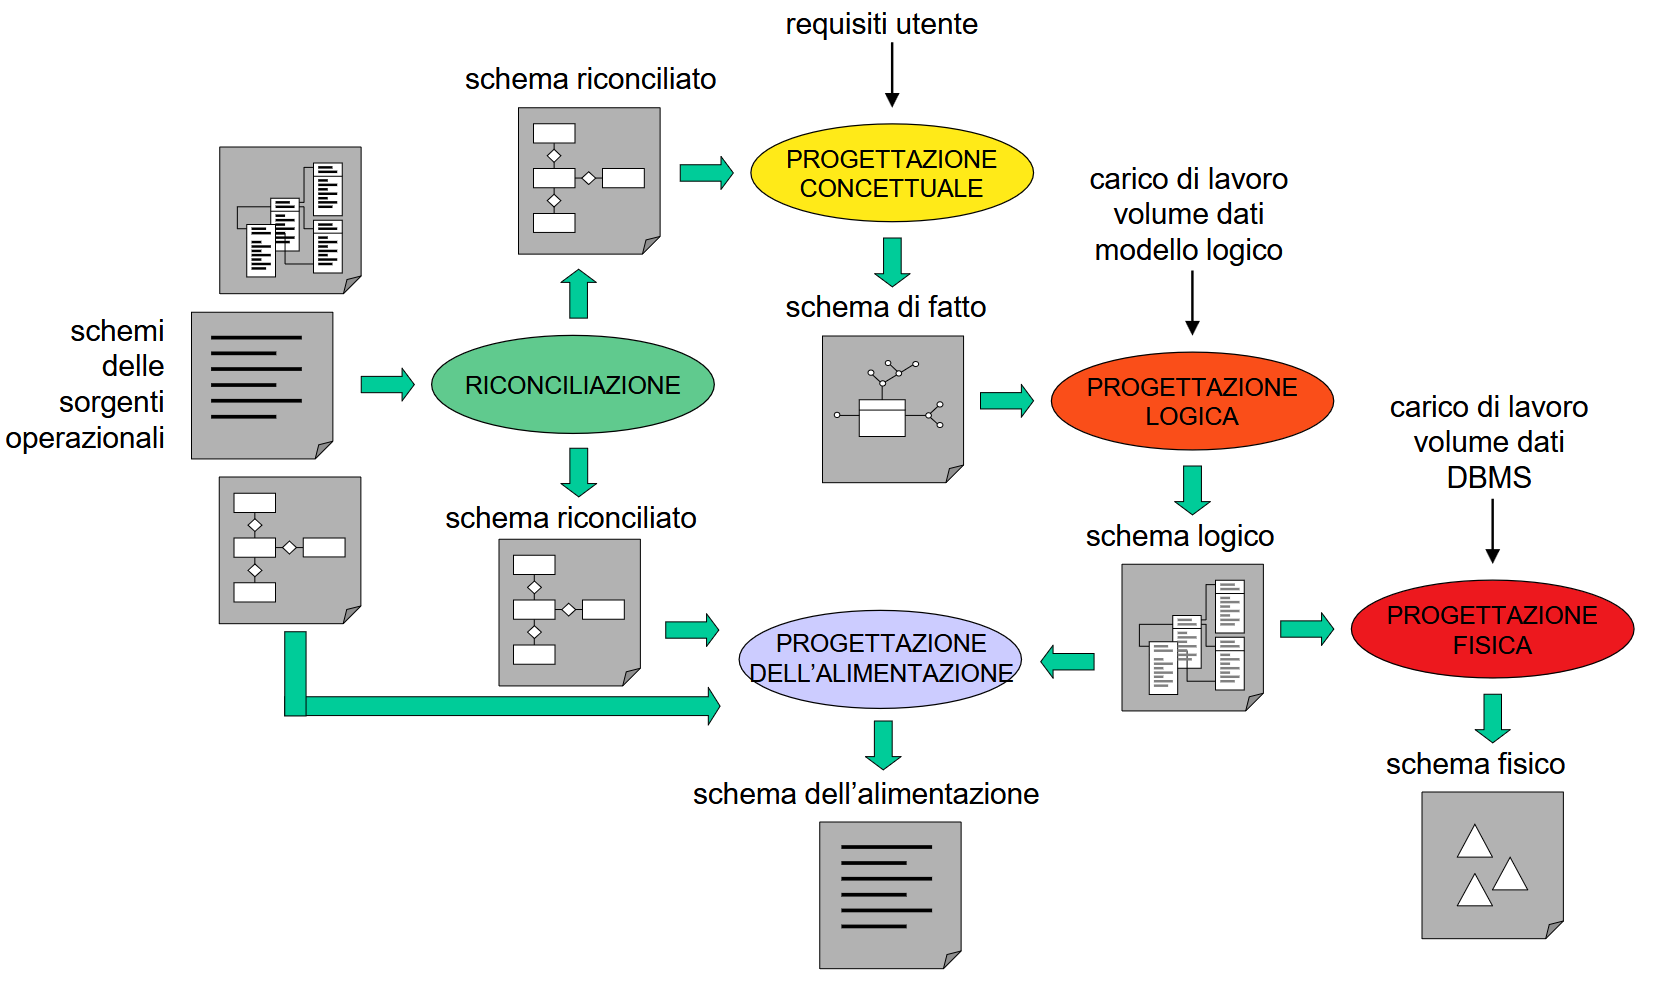
\includegraphics[width=0.75\textwidth]{capitoli/03_Data warehouse_progettazione concettuale e logica/images/approccio_bottom_up.png}
    \caption{Approccio Bottom-Up: si parte da un data mart specifico e si procede all'integrazione con altri data mart per formare il data warehouse completo.}
\end{figure}

\section{Analisi dei Requisiti}

Il processo di realizzazione di un data mart (approccio bottom-up) inizia sempre dall'analisi dei requisiti. Si tratta di comprendere quali sono le analisi di interesse per gli attori di business (che variano a seconda del ruolo, es. direttore vendite vs capo del personale) e identificare i dati necessari per supportarle. 

La raccolta dei requisiti avviene tipicamente tramite \textbf{interviste} che coinvolgono sia i \textit{business users} (utilizzatori finali) sia gli amministratori del sistema informativo. Di norma, il primo data mart sviluppato riguarda un settore strategico dell'azienda per dimostrare fin da subito l'efficacia del progetto.

La progettazione si basa su tre pilastri (pillar) fortemente interconnessi:
\begin{enumerate}
    \item \textbf{Tecnologia:} Quale DBMS usare, spazio di archiviazione, livello di affidabilità.
    \item \textbf{Dati:} Quali dati servono, se sono presenti nelle sorgenti interne o se vanno integrati con fonti esterne, e come effettuare l'integrazione.
    \item \textbf{Applicazioni:} Che tipo di applicativo utilizzerà l'utente finale (dashboard interattiva, algoritmi predittivi, soluzioni agentiche basate su LLM/RAG). La tecnologia scelta deve supportare l'applicazione desiderata.
\end{enumerate}

I requisiti si dividono in due grandi categorie: applicativi e strutturali.

\subsection{Requisiti Applicativi}
Definiscono il "che cosa" si vuole analizzare.
\begin{itemize}
    \item \textbf{Descrizione degli eventi di interesse (Fatti):} Un fatto rappresenta una categoria di eventi aziendali (es. reclami, quantità venduta, giacenze di magazzino). È caratterizzato da coordinate di analisi (dimensioni) e da indicatori numerici (misure o KPI).
    \item \textbf{Carico di lavoro:} Quali e quanti attori accedono al sistema, la frequenza di generazione dei report, il numero di sessioni in contemporanea. Queste informazioni permettono di dimensionare opportunamente il sistema.
\end{itemize}

\subsection{Requisiti Strutturali}
Riguardano l'infrastruttura e i vincoli operativi.
\begin{itemize}
    \item \textbf{Periodicità dell'alimentazione:} Il data warehouse necessita di un caricamento periodico (ETL). Solitamente avviene nelle ore notturne, quando il carico dei sistemi informativi e del data warehouse è minimo.
    \item \textbf{Spazio disponibile:} Sia per i dati grezzi che per strutture accessorie necessarie a velocizzare le interrogazioni (indici, viste materializzate).
    \item \textbf{Tipo di architettura:} A due o tre livelli, e definizione se i data mart saranno dipendenti (condividono dimensioni di analisi) o indipendenti.
\end{itemize}

\section{Progettazione Concettuale: Dimensional Fact Model (DFM)}

Dopo aver raccolto i requisiti (e aver definito uno schema riconciliato delle sorgenti nel caso di sistemi informativi eterogenei), si passa alla progettazione concettuale. In questo ambito, il \textbf{modello Entità-Relazione (ER) non è adatto}.
Il modello ER nasce per i DBMS operazionali: il suo scopo è normalizzare i dati per evitare ridondanze e prevenire anomalie di aggiornamento. Tuttavia, uno schema normalizzato frammenta l'informazione; per ricostruirla in fase di interrogazione analitica (su milioni di record) sarebbero necessarie numerose operazioni di \texttt{JOIN}, rendendo il sistema inefficiente.

Nel data warehouse \textbf{rinunciamo alla normalizzazione e accettiamo la ridondanza} per ottenere query efficienti. Il modello concettuale di riferimento è il \textbf{Dimensional Fact Model (DFM)}, introdotto da Golfarelli e Rizzi, che offre una rappresentazione grafica basata su fatti, dimensioni e misure.

\subsection{Elementi Base del DFM}

\begin{itemize}
    \item \textbf{Fatto:} Modella un insieme di eventi di interesse (es. vendite). Nel DFM è rappresentato dal nodo centrale. Solitamente, in un modello ER equivalente, il fatto rappresenta una relazione molti-a-molti (ennaria) tra tutte le dimensioni coinvolte (es. lo stesso prodotto può essere venduto in più negozi e in più date).
    \item \textbf{Dimensione:} Descrive le coordinate di analisi di un fatto (es. Negozio, Prodotto, Data). Le dimensioni sono tendenzialmente ortogonali tra loro.
    \item \textbf{Misura (o Metrica):} Una proprietà numerica associata al fatto, oggetto di operazioni di aggregazione (es. quantità venduta, incasso, numero di clienti).
    \item \textbf{Gerarchia:} Sulle dimensioni è possibile definire delle gerarchie (es. Data $\rightarrow$ Mese $\rightarrow$ Trimestre $\rightarrow$ Anno). Esse rappresentano generalizzazioni di concetti e modellano una \textbf{dipendenza funzionale} (relazione 1:N). 
\end{itemize}

\subsubsection{Le Gerarchie e le Dipendenze Funzionali}
Nel DFM, un arco in una gerarchia rappresenta una dipendenza funzionale, ovvero, dato l'attributo di partenza, esiste \textit{uno e un solo} valore per l'attributo di destinazione. 
L'arco va tracciato solo verso l'attributo meno generale immediatamente successivo. Ad esempio, esiste una dipendenza funzionale tra \textit{Data} e \textit{Anno}, ma l'arco viene disegnato da \textit{Data} a \textit{Mese}, e da \textit{Mese} a \textit{Trimestre}, e da quest'ultimo ad \textit{Anno}.
Inoltre, non si traccia un arco tra \textit{Giorno della settimana} (lunedì, martedì...) e \textit{Anno}, perché un "lunedì" non appartiene univocamente a un solo anno (non c'è dipendenza funzionale 1:N).

Un'attenzione particolare va posta al concetto temporale nel business: quando si parla di "analisi per mese", si intende quasi sempre il mese in un determinato anno (es. Settembre 2026), distinto dal mese di un altro anno. Se l'obiettivo fosse analizzare tutti i mesi di settembre a prescindere dall'anno, si parlerebbe di "mese dell'anno".

% FIGURA ORIGINALE DA RECUPERARE DALLE SLIDE
% Slide di provenienza: 11
% Tipo: schema
% Descrizione: Rappresentazione grafica di un Dimensional Fact Model (DFM) di base con il fatto Vendita, dimensioni, gerarchie e misure.
% Punto di inserimento: Qui, per mostrare un esempio di schema DFM.
% File da inserire: dfm_base_vendita.png
\begin{figure}[H]
    \centering
    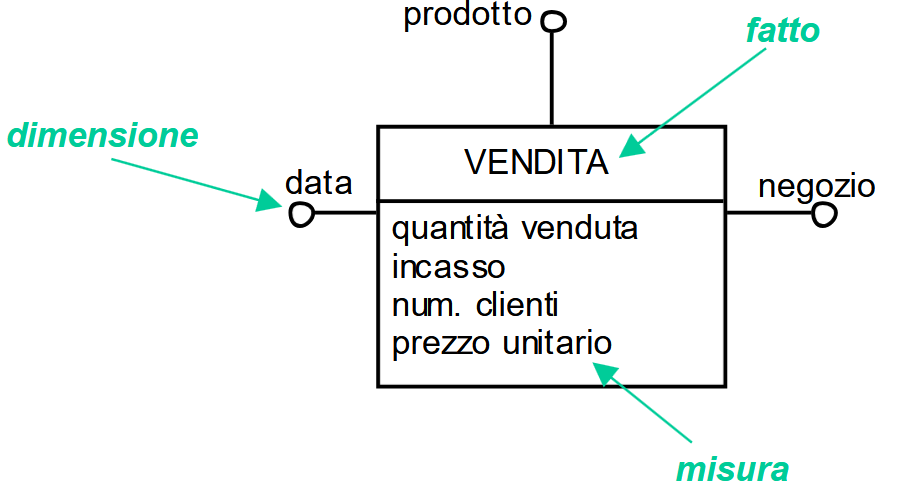
\includegraphics[width=0.6\textwidth]{capitoli/03_Data warehouse_progettazione concettuale e logica/images/dfm_base_vendita.png}
    \caption{Esempio di Dimensional Fact Model per le vendite, con dimensioni (Negozio, Prodotto, Data), gerarchie (es. Negozio $\rightarrow$ Città) e misure (Qta, Incasso).}
    \label{fig:dfm-base}
\end{figure}

\subsection{Confronto: DFM vs Modello ER}
Se traducessimo un fatto in un modello ER, esso diventerebbe un'entità associativa centrale che collega con relazioni N:1 le varie entità dimensionali, le quali a loro volta si esploderebbero a cascata a causa delle dipendenze funzionali (gerarchie) in una miriade di tabelle (forma normale). Il DFM "collassa" visivamente e logicamente queste gerarchie.

% FIGURA ORIGINALE DA RECUPERARE DALLE SLIDE
% Slide di provenienza: 14
% Tipo: diagramma
% Descrizione: Confronto tra uno schema DFM e il corrispondente modello ER altamente normalizzato.
% Punto di inserimento: Qui, a supporto della spiegazione sul superamento del modello ER.
% File da inserire: dfm_vs_er.png
\begin{figure}[H]
    \centering
    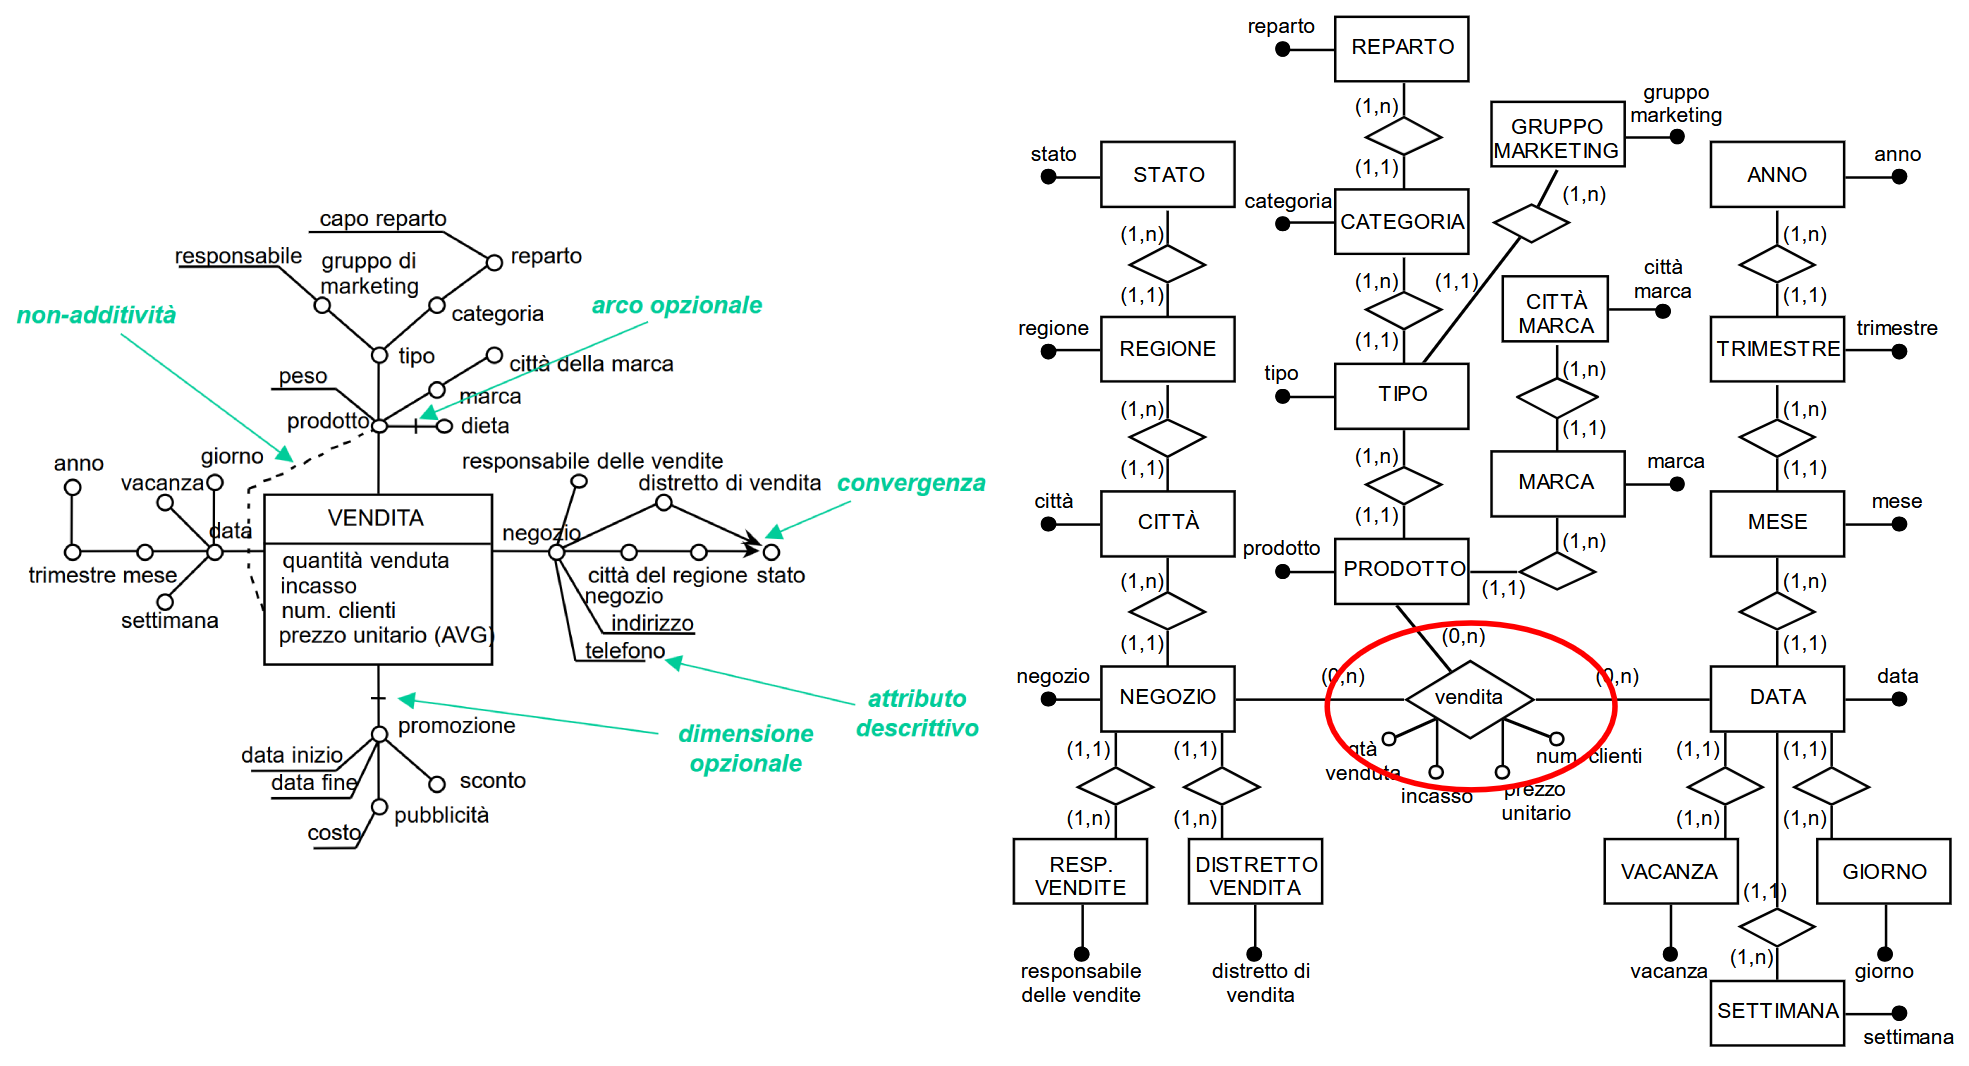
\includegraphics[width=0.95\textwidth]{capitoli/03_Data warehouse_progettazione concettuale e logica/images/dfm_vs_er.png}
    \caption{Confronto tra la notazione compatta del DFM (a sinistra) e la complessità di un modello ER equivalente (a destra) dove tutte le dipendenze funzionali sono esplicitate in tabelle separate.}
    \label{fig:dfm-vs-er}
\end{figure}

\section{Misure e Operatori di Aggregazione}

Il processo tipico in un data warehouse è l'analisi a diversi livelli di dettaglio, che corrisponde in SQL all'applicazione della clausola \texttt{GROUP BY} navigando lungo le gerarchie. È fondamentale capire quali misure possono essere aggregate e come.

\subsection{Classificazione delle Misure}
Le metriche si dividono in tre categorie in base alla loro additività (la capacità di essere sommate lungo le dimensioni, specialmente il tempo):

\begin{enumerate}
    \item \textbf{Misure di flusso:} Possono essere valutate cumulativamente alla fine di un periodo di tempo. Sono \textbf{sempre additive} lungo tutte le dimensioni.
    \begin{itemize}
        \item \textit{Esempi:} Quantità di prodotti venduti, importo incassato. Se vendo 10 oggetti oggi e 20 domani, in totale ho venduto 30 oggetti.
    \end{itemize}
    \item \textbf{Misure di livello:} Rappresentano un'istantanea (snapshot) di un fenomeno in un preciso istante di tempo. \textbf{Non sono additive lungo la dimensione temporale}.
    \begin{itemize}
        \item \textit{Esempi:} Giacenza di magazzino, saldo del conto corrente. Se oggi ho 100€ sul conto e domani ho 100€, la somma 200€ non ha alcun significato; il valore "fotografa" lo stato attuale. Tuttavia, \textit{possono} essere additive lungo lo spazio (es. somma delle giacenze di tre magazzini diversi nello stesso istante).
    \end{itemize}
    \item \textbf{Misure unitarie:} Valutate in specifici istanti ed espresse in termini relativi. \textbf{Non sono additive} lungo nessuna dimensione.
    \begin{itemize}
        \item \textit{Esempio:} Prezzo unitario di un prodotto.
    \end{itemize}
\end{enumerate}

Un'ulteriore eccezione all'additività si ha quando l'aggregazione su una dimensione genera duplicati di conteggio. Ad esempio, la metrica \textit{Numero Clienti} calcolata come numero di scontrini: è sommabile nel tempo, ma \textbf{non è additiva rispetto ai Prodotti}. Poiché uno stesso cliente può comprare più prodotti in uno stesso scontrino, aggregare i clienti per prodotto porterebbe a contare la stessa persona più volte (overlap). Sul DFM questa non-additività va esplicitata graficamente.

\subsection{Operatori di Aggregazione}
A seconda di come è possibile calcolare aggregazioni partendo da dati già pre-aggregati a un livello di dettaglio maggiore, gli operatori si classificano in:

\begin{itemize}
    \item \textbf{Distributivi:} Il calcolo finale può sfruttare risultati aggregati intermedi. (es. \texttt{SUM}, \texttt{MIN}, \texttt{MAX}). 
    \textit{Esempio:} Per calcolare le vendite annuali, posso sommare i parziali delle vendite trimestrali già calcolati. Questo abbassa drasticamente i tempi di calcolo.
    \item \textbf{Algebrici:} Il risultato intermedio da solo non basta, ma è possibile calcolarlo se affiancato da misure di supporto. (es. \texttt{AVG}).
    \textit{Motivazione:} La media delle medie è matematicamente scorretta. Per aggregare una media a un livello superiore, il data warehouse non dovrebbe memorizzare la "media" come metrica secca, ma memorizzare le metriche di base che la compongono (es. l'incasso e il numero di prodotti) per ricalcolarla in SQL come \texttt{SUM(Incasso) / SUM(Num\_Prodotti)}.
    \item \textbf{Olistici:} Non è possibile sfruttare alcun aggregato parziale; è necessario ricalcolare la funzione partendo dai dati originali di massimo dettaglio. (es. Moda, Mediana).
\end{itemize}

\section{Costrutti Avanzati nel DFM}

La modellazione concettuale deve saper gestire casi della realtà aziendale più complessi.

\subsection{Attributi Descrittivi e Gerarchie Condivise}
\begin{itemize}
    \item \textbf{Attributi descrittivi:} Sono caratteristiche associate a una dimensione su cui però \textit{non si fanno aggregazioni} (es. Indirizzo, Telefono del negozio). Si rappresentano graficamente con una linea semplice (senza cerchio).
    \item \textbf{Gerarchia Condivisa:} Spesso una stessa dimensione assume "ruoli" multipli nello stesso fatto. L'esempio classico è il traffico telefonico: una chiamata ha un \textit{Numero Chiamante} e un \textit{Numero Chiamato}. Entrambi puntano all'entità Numero Telefonico (che possiede una sua gerarchia, es. Distretto, Uso). Nel DFM si tracciano due frecce separate dal Fatto alla dimensione, specificando il ruolo su ciascuna freccia. Altri esempi: aeroporto di partenza e destinazione in un volo; mittente e destinatario in una spedizione o in un bonifico.
\end{itemize}

\subsection{L'Arco Multiplo}
Come abbiamo visto, la gerarchia modella dipendenze funzionali 1:N. Ma cosa succede quando tra due attributi dimensionali esiste una \textbf{relazione Molti-a-Molti}?
Si utilizza l'arco multiplo, rappresentato da due linee convergenti.

\textbf{Casi d'uso:}
\begin{enumerate}
    \item \textbf{Libri e Autori:} Vogliamo analizzare le vendite di libri. Un libro può essere scritto da più autori, un autore scrive più libri. Date le vendite del "Libro X", ad esso è associato un numero indefinito di autori.
    \item \textbf{Ricoveri e Diagnosi:} Un paziente in pronto soccorso può avere un "Gruppo di diagnosi" che racchiude $N$ patologie diverse. Associando il costo del ricovero all'intero gruppo (più specifico) e connettendo il gruppo alla singola diagnosi (tramite arco multiplo), semplifichiamo il calcolo del costo evitando di duplicarlo o distribuirlo in modo arbitrario tra le singole patologie.
\end{enumerate}

L'arco multiplo è obbligatorio quando non si conosce a priori il numero massimo di valori (es. numero di autori di un libro) oppure quando tale numero è grande.

\subsection{L'Attributo Configurazione}
Se abbiamo un attributo multivalore (come l'arco multiplo) ma \textbf{conosciamo a priori i valori ammissibili e questi sono pochi (generalmente $\le 10$)}, possiamo semplificare notevolmente il modello.
Invece di creare un nodo separato e richiedere complessi \texttt{JOIN}, inseriamo nel modello un \textbf{Attributo Configurazione}. 

\textit{Funzionamento:} Si "esplode" l'informazione creando un attributo booleano (Sì/No) per ciascun valore possibile. 
\textit{Esempi:}
\begin{itemize}
    \item Un negozio di videogame che può vendere 4 specifiche tipologie di giochi. Avremo 4 campi booleani nel record del negozio.
    \item Le università e l'elenco dei servizi gratuiti (Wi-Fi, Sale studio, Mensa). Se i servizi mappati sono meno di 10, usiamo una configurazione.
\end{itemize}
Questo costrutto rende le query analitiche molto più semplici, potendo filtrare direttamente con predicati booleani nella clausola \texttt{WHERE}.

% FIGURA ORIGINALE DA RECUPERARE DALLE SLIDE
% Slide di provenienza: 21 e 22
% Tipo: schema
% Descrizione: Esempi di costrutti avanzati del DFM: Arco Multiplo (Libro-Autore) e Attributo Configurazione (Categorie di videogame).
% Punto di inserimento: Qui, per visualizzare le alternative descritte sopra.
% File da inserire: dfm_costrutti_avanzati.png
\begin{figure}[H]
    \centering
    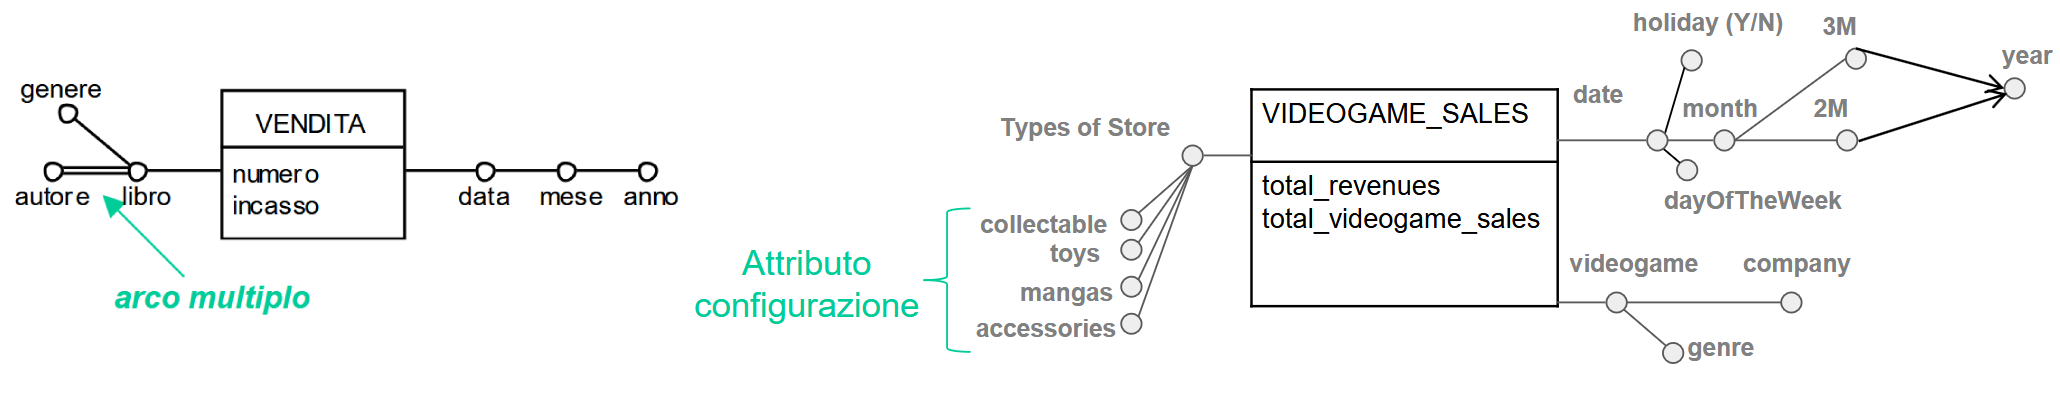
\includegraphics[width=0.9\textwidth]{capitoli/03_Data warehouse_progettazione concettuale e logica/images/dfm_costrutti_avanzati.png}
    \caption{Rappresentazione di un arco multiplo (a sinistra) e di un attributo configurazione (a destra) nel Dimensional Fact Model.}
    \label{fig:dfm-costrutti-avanzati}
\end{figure}

\subsection{Schemi di Fatto Vuoti}
Non tutti i fatti registrano valori monetari o metriche di flusso. Se l'obiettivo è memorizzare \textbf{la pura presenza/verificarsi di un evento}, creiamo uno \textit{schema di fatto vuoto}, ovvero privo di misure.
\textit{Esempio:} La frequenza degli studenti ai corsi. L'evento è caratterizzato dalle dimensioni Studente, Semestre, Corso. Se la tripla esiste nel Data Warehouse, l'evento si è verificato. In questo caso, l'unico operatore di aggregazione applicabile nelle query è il \texttt{COUNT(*)} per contare gli eventi accaduti.

\section{La Rappresentazione del Tempo (Slowly Changing Dimensions)}

Il data warehouse conserva lo storico aziendale. I fatti sono intrinsecamente legati al tempo (dimensione Data), ma anche gli attributi delle altre dimensioni possono subire \textbf{variazioni lente nel tempo} (Slowly Changing Dimensions - SCD), ad esempio un cliente che cambia stato civile, o un prodotto che cambia nome o packaging.
Gestire questi cambiamenti è vitale per non falsare le analisi. Esistono tre modalità (o Tipi) principali:

\subsection{Rappresentazione di Tipo 1 (Sovrascrittura)}
È la fotografia dell'istante attuale. Il valore vecchio viene \textbf{sovrascritto} con quello nuovo.
\begin{itemize}
    \item \textit{Esempio:} Il cliente Mario Rossi si sposa. Lo stato civile viene sovrascritto. Tutti gli acquisti fatti da single figurano ora come fatti da "sposato". Anche un prodotto (es. cereali) che cambia nome, assocerebbe tutte le vendite passate al nuovo nome.
    \item \textit{Problema:} Si perde totalmente la memoria storica e la correlazione tra l'evento temporale (il cambio) e i volumi. In contesti reali è fortemente sconsigliato.
\end{itemize}

\subsection{Rappresentazione di Tipo 2 (Nuova Istanza)}
Per ogni variazione si crea un \textbf{nuovo record (istanza)} della dimensione.
\begin{itemize}
    \item \textit{Esempio:} Avremo due record distinti: "Mario Rossi Single" e "Mario Rossi Sposato". Gli eventi passati sono legati al primo, i nuovi al secondo.
    \item \textit{Problema:} I due record sono trattati dal sistema come entità indipendenti (come fossero due persone o due prodotti diversi). Non si può fare un'analisi aggregata che confronti facilmente "il prima e il dopo" per lo stesso soggetto senza complessi artifici.
\end{itemize}

\subsection{Rappresentazione di Tipo 3 (Campionamento Temporale)}
È l'approccio più completo e raccomandato, che richiede una modifica dello schema della dimensione. Oltre a creare una nuova istanza, si introducono attributi di validità e sequenzialità:
\begin{itemize}
    \item Una coppia di \textit{timestamp} (\texttt{inizio\_validità}, \texttt{fine\_validità}).
    \item Un identificativo di sequenza (o master ID) che lega tra loro tutte le incarnazioni della stessa entità logica.
\end{itemize}
In questo modo, quando Mario Rossi si sposa, la validità della prima istanza viene chiusa, se ne apre una nuova lo stesso giorno, ed entrambe puntano al medesimo soggetto reale, permettendo al sistema di ricostruire l'esatta storia dimensionale.

\begin{table}[htbp]
    \centering
    \caption{Esempio di gestione di una variazione dimensionale con il Tipo 3}
    \label{tab:scd-tipo3}
    \begin{tabular}{|c|c|l|c|c|c|}
        \hline
        \textbf{ID record} & \textbf{Master ID} & \textbf{Cliente} & \textbf{Stato civile} & \textbf{Inizio validità} & \textbf{Fine validità} \\
        \hline
        101 & 25 & Mario Rossi & Single & 01/01/2022 & 14/06/2024 \\
        \hline
        248 & 25 & Mario Rossi & Sposato & 15/06/2024 & -- \\
        \hline
    \end{tabular}
\end{table}

Il campo \textit{Master ID} identifica la stessa entità logica nelle sue diverse
istanze, mentre le date delimitano il periodo in cui ciascun record è valido.


\section{Dimensionamento del Data Warehouse: Carico di Lavoro e Volume dei Dati}

Durante la progettazione è necessario stimare lo spazio occupato su disco e le performance. Il calcolo del volume massimo teorico dei dati è dato dal \textbf{prodotto cartesiano delle cardinalità} di tutte le dimensioni. 
Tuttavia, le dimensioni nei modelli data warehouse sono considerate ortogonali, ma nella realtà fisica esiste la \textbf{sparsità}.

\subsection{La Sparsità dei Dati}
La sparsità indica la densità effettiva dei dati rispetto alle combinazioni teoriche. 
Se abbiamo le dimensioni Data, Fascia Oraria, Negozio e Prodotto: non è realistico ipotizzare che \textit{tutti} i prodotti a catalogo vengano venduti in \textit{tutti} i negozi, \textit{tutti} i giorni, in \textit{tutte} le fasce orarie.
Se la combinazione massima è 10.000, e si stima che solo il 15\% dei prodotti venga effettivamente venduto con questa frequenza, il fattore di sparsità interviene per ridurre la stima.

\textbf{Legge dell'aggregazione:} La sparsità si riduce al crescere del livello di aggregazione dei dati. Se passiamo dall'analisi per "Singola Data e Fascia oraria" all'analisi per "Mese", un prodotto che non era venduto tutti i giorni molto probabilmente verrà venduto almeno una volta nel corso dell'intero mese. Di conseguenza, salendo nella gerarchia, la matrice dei dati diventa molto più "densa" e la probabilità che l'evento si verifichi si avvicina al 100\%.

Questo è il motivo principale per cui i data warehouse \textbf{non vengono implementati utilizzando fisicamente matrici n-dimensionali} pure. In una matrice, lo spazio per l'evento viene allocato in memoria che esso si verifichi o meno, sprecando enormi quantità di spazio. Si preferisce usare il \textbf{modello Relazionale (ROLAP)}, dove il record viene scritto (occupando spazio) solo se l'evento è realmente accaduto.

\begin{figure}[H]
    \centering
    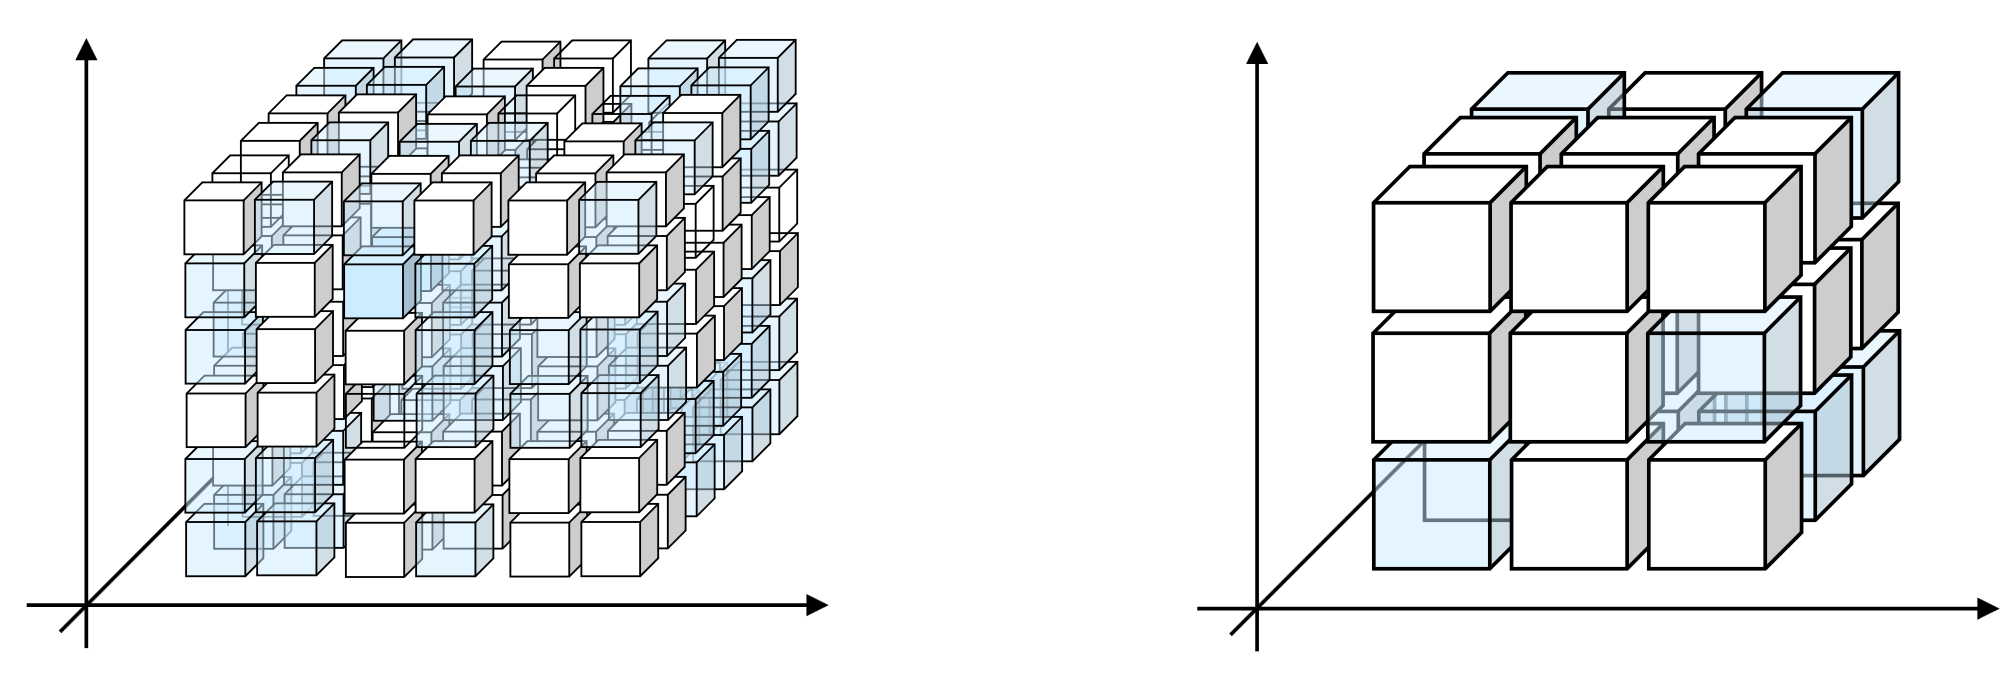
\includegraphics[width=0.7\textwidth]{capitoli/03_Data warehouse_progettazione concettuale e logica/images/sparsita.png}
    \caption{Esempio di sparsità dei dati: la matrice teorica (a sinistra) mostra tutte le combinazioni possibili, mentre la matrice reale (a destra) evidenzia solo le combinazioni effettivamente verificatesi.}
    \label{fig:sparsita}
\end{figure}

\section{Progettazione Logica: Il Modello Relazionale per il Data Warehouse}

La progettazione logica produce uno \textbf{schema logico relazionale (ROLAP)} partendo dal modello concettuale DFM. Si basa su due princìpi opposti rispetto ai database tradizionali:
1. Denormalizzazione delle tabelle.
2. Tolleranza (e ricerca) della ridondanza dei dati per ottimizzare i tempi di lettura.

\subsection{Lo Schema a Stella (Star Schema)}
È l'architettura standard per i data warehouse relazionali.
\begin{itemize}
    \item \textbf{Tabelle delle Dimensioni:} Si crea \textit{una sola tabella per dimensione}. Le gerarchie vengono schiacciate e perse a livello strutturale: gli attributi di diverso livello (es. Data, Mese, Anno) diventano colonne della medesima tabella, generando forte ridondanza (es. il mese e l'anno saranno ripetuti identici per ogni giorno di quel mese).
    La \textbf{Chiave Primaria} della tabella dimensionale è sempre una chiave generata artificialmente (\textbf{chiave surrogata}, un contatore intero), mai una stringa o una logica di business, per velocizzare le operazioni di \texttt{JOIN}.
    \item \textbf{Tabella dei Fatti:} Si crea al centro dello schema. Contiene come chiavi esterne le chiavi surrogate delle dimensioni e, come attributi diretti, tutte le misure.
\end{itemize}

% FIGURA ORIGINALE DA RECUPERARE DALLE SLIDE
% Slide di provenienza: 34
% Tipo: diagramma ER
% Descrizione: Diagramma E-R che mostra la struttura di uno Star Schema (Fatto al centro, Dimensioni intorno).
% Punto di inserimento: Qui, per illustrare lo Schema a Stella.
% File da inserire: star_schema.png
\begin{figure}[H]
    \centering
    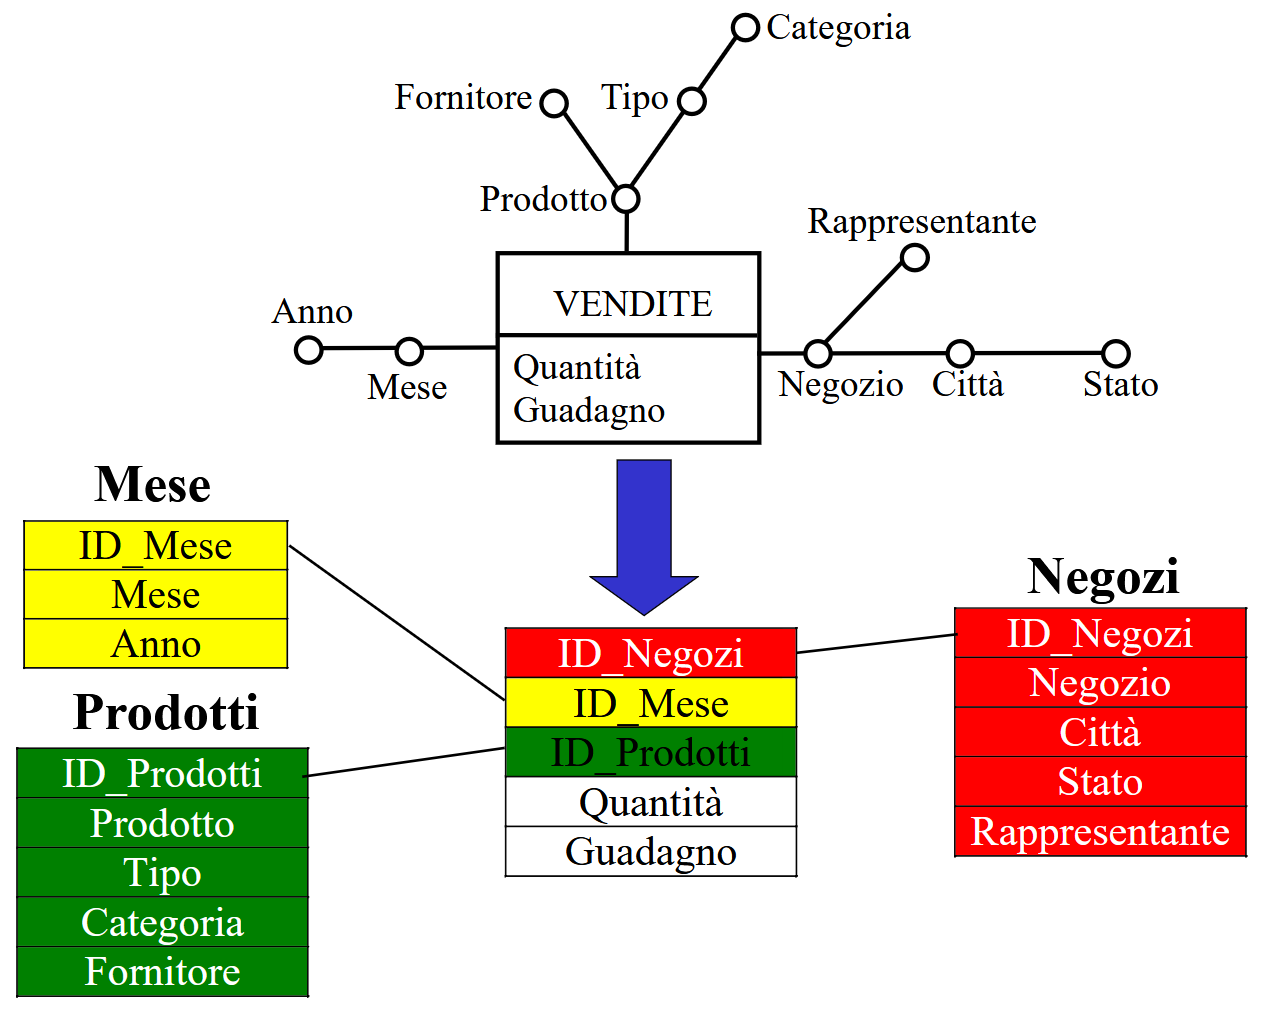
\includegraphics[width=0.75\textwidth]{capitoli/03_Data warehouse_progettazione concettuale e logica/images/star_schema.png}
    \caption{Struttura di uno Schema a Stella (Star Schema): il fatto centrale è circondato da tabelle dimensionali completamente denormalizzate.}
    \label{fig:star-schema}
\end{figure}

\subsection{Lo Schema a Fiocco di Neve (Snowflake Schema)}
Lo \textit{Snowflake Schema} tenta di reinserire la normalizzazione nello Star Schema. Sostanzialmente, si "taglia" una gerarchia dimensionale mettendola in una tabella separata (es. separando la gerarchia geografica dalla tabella Negozio).
\begin{itemize}
    \item \textbf{Difetti:} Il risparmio di spazio su disco è marginale (perché le tabelle dimensionali sono trascurabili rispetto ai milioni di record della tabella dei fatti). In compenso, per ricostruire l'informazione il sistema dovrà eseguire \texttt{JOIN} aggiuntivi, degradando le prestazioni.
    \item \textbf{Uso reale:} Lo schema Snowflake è fortemente sconsigliato e raramente utilizzato nella pratica aziendale.
\end{itemize}

\begin{figure}[H]
    \centering
    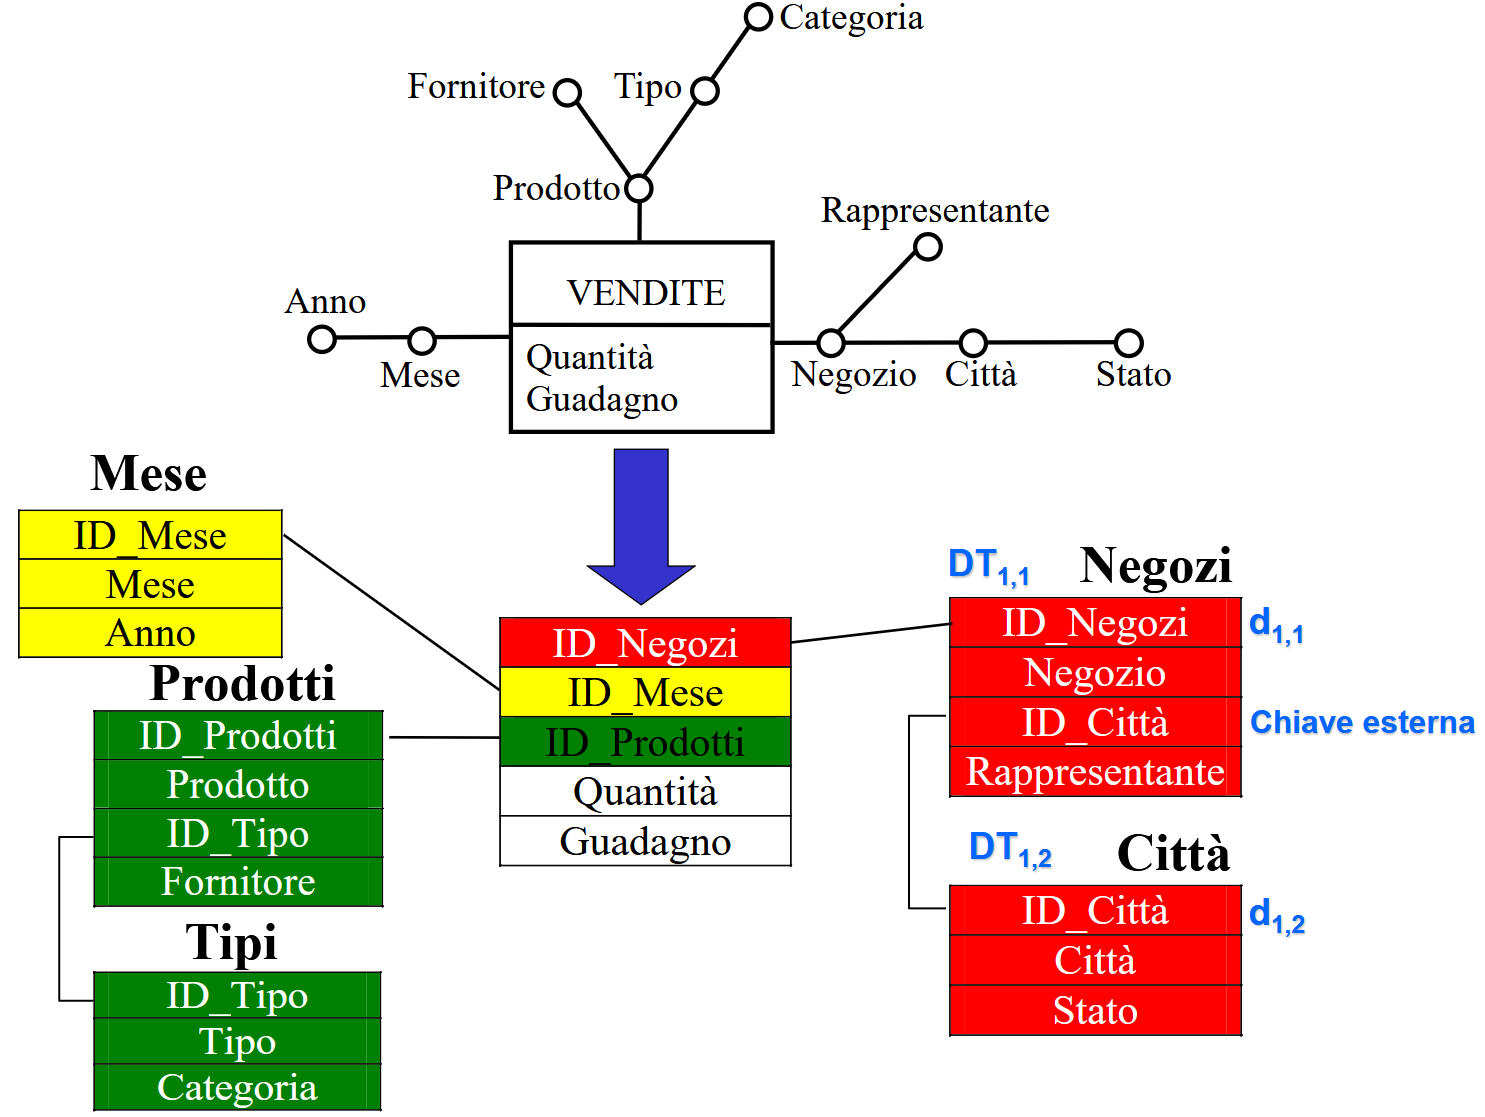
\includegraphics[width=0.75\textwidth]{capitoli/03_Data warehouse_progettazione concettuale e logica/images/snowflake_schema.png}
    \caption{Struttura di uno Schema a Fiocco di Neve (Snowflake Schema): la gerarchia geografica è separata dalla tabella Negozio, richiedendo un join aggiuntivo per ricostruire l'informazione.}
    \label{fig:snowflake-schema}
\end{figure}

\subsection{Traduzione Logica degli Archi Multipli}
Come si mappa l'arco multiplo (relazione N:M tra dimensioni) in un database relazionale? Esistono due soluzioni principali (oltre a quella dell'attributo configurazione già discussa):

\begin{enumerate}
    \item \textbf{Bridge Table (Tabella Ponte):} È la soluzione più ortodossa. Si crea una tabella intermedia tra il Fatto e la Dimensione multiautore (es. tra Vendita Libro e Autore). Questa tabella modella le coppie valide e introduce un \textbf{Peso} (es. 0.5 se gli autori sono due).
    \begin{itemize}
        \item \textit{Pro:} Permette interrogazioni pesate corrette (es. dividere l'incasso del libro equamente tra gli autori: \texttt{SUM(Incasso * Peso)}).
        \item \textit{Contro:} Rende complesse le query di semplice impatto (es. "Quante copie ha venduto l'autore in totale, a prescindere dal co-autoraggio?") e introduce un overhead di join.
    \end{itemize}
    \item \textbf{Push Down:} L'arco multiplo viene "spinto" direttamente nella Tabella dei Fatti. Il Fatto viene sdoppiato/moltiplicato: se un libro ha 3 autori, si creano 3 record nella tabella dei fatti, ognuno puntante a un autore diverso.
    \begin{itemize}
        \item \textit{Pro:} Costo di interrogazione bassissimo (elimina il join aggiuntivo).
        \item \textit{Contro:} Moltiplica enormemente lo spazio occupato dalla Tabella dei Fatti (che è già enorme). L'incasso andrebbe pre-frazionato (calcolato) durante la fase di ETL prima dell'inserimento, rendendo difficili eventuali variazioni. Le interrogazioni "di impatto" (senza frazionamento) diventano molto pericolose per il rischio di doppie somme.
    \end{itemize}
\end{enumerate}

\begin{figure}[H]
    \centering
    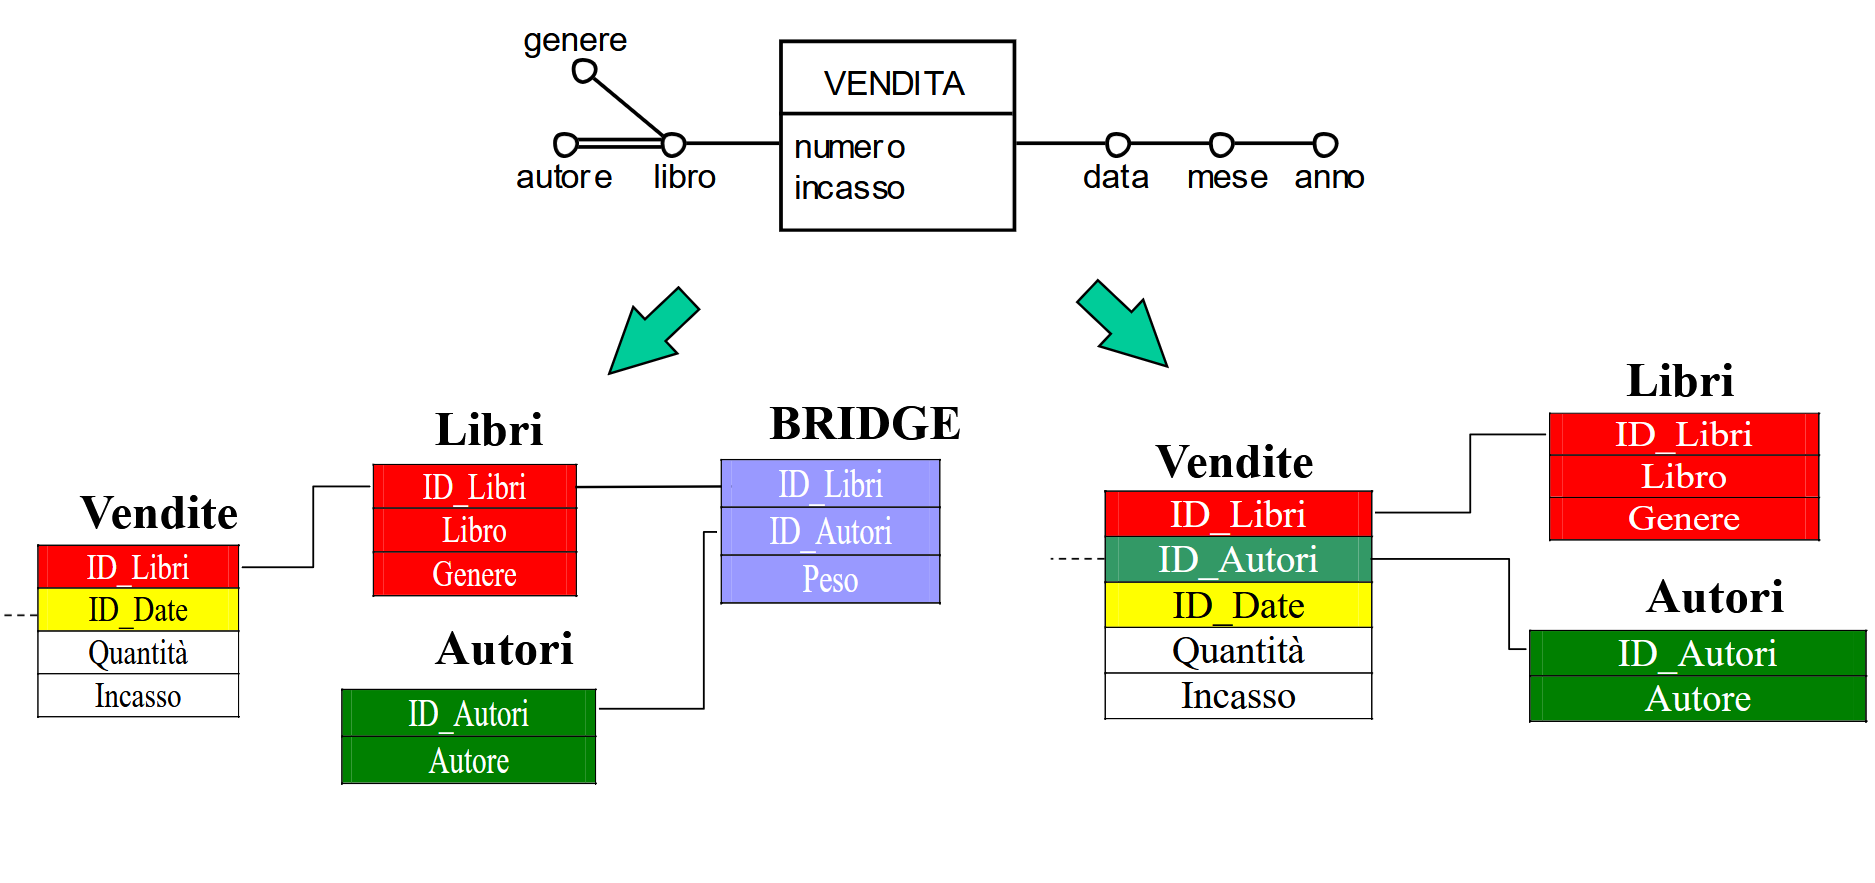
\includegraphics[width=0.75\textwidth]{capitoli/03_Data warehouse_progettazione concettuale e logica/images/archi_multipli.png}
    \caption{Traduzione logica di un arco multiplo: a sinistra la soluzione con Bridge Table, a destra la soluzione Push Down.}
    \label{fig:archi-multipli}
\end{figure}

\subsection{Dimensioni Degeneri e Junk Dimension}
Una dimensione è \textit{degenere} quando, dopo l'analisi, risulta composta da un \textbf{solo attributo} (privo di gerarchie). 
Per mappare queste dimensioni logicamente, esistono due vie:
\begin{enumerate}
    \item \textbf{Integrazione nella Tabella dei Fatti:} (Push down). L'attributo viene inserito come normale colonna all'interno del Fatto, senza creare una tabella dimensionale esterna.
    \item \textbf{Junk Dimension (Dimensione "pattumiera"):} Se ci sono molte dimensioni degeneri scorrelate (es. flag di stato, tipi di spedizione, codici semplici), le si compatta tutte in un'unica dimensione artificiale che contiene il \textit{prodotto cartesiano} di tutte le combinazioni possibili di questi attributi. Nella tabella dei fatti risiederà solo un ID puntatore a questa riga. Questa soluzione è adottabile solo se la cardinalità risultante (le combinazioni totali) rimane piccola.
\end{enumerate}


\begin{figure}
    \centering
    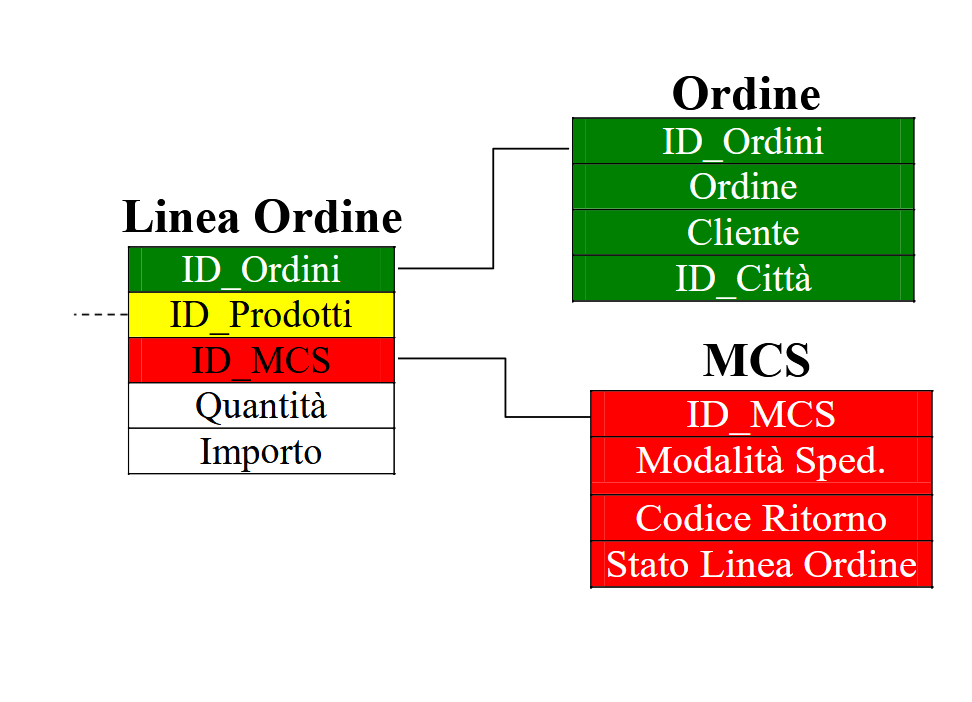
\includegraphics[width=0.75\textwidth]{capitoli/03_Data warehouse_progettazione concettuale e logica/images/junk_dimension.png}
    \caption{Esempio di Junk Dimension: le dimensioni degeneri "Tipo Spedizione" e "Flag Stato" vengono combinate in un'unica tabella dimensionale, riducendo il numero di join nella Tabella dei Fatti.}
    \label{fig:junk-dimension}
\end{figure}
% ==============================================================================
% FINE DISPENSA
% ==============================================================================
\chapter{Analisi dei Data Warehouse}


\chapter{Progettazione Fisica e Alimentazione del Data Warehouse}

\section{Progettazione Fisica}
La progettazione logica di una base di dati definisce uno schema indipendente da come le informazioni vengono effettivamente memorizzate sul disco, garantendo così l'indipendenza logica. La progettazione fisica, al contrario, ha l'obiettivo di definire le strutture fisiche di memorizzazione e di accesso ai dati al fine di ottimizzare i tempi di esecuzione delle interrogazioni. 
Poiché SQL è un linguaggio dichiarativo (si specifica \textit{cosa} cercare e non \textit{come}), spetta a un modulo interno del DBMS, chiamato \textbf{ottimizzatore}, decidere il piano di esecuzione più efficiente. Il compito del progettista fisico è quindi fornire all'ottimizzatore le strutture accessorie adeguate.

\subsection{Caratteristiche del carico di lavoro nel Data Warehouse}
I sistemi di Data Warehouse sono progettati per soddisfare specifiche esigenze di analisi. Il carico di lavoro tipico presenta le seguenti caratteristiche:
\begin{itemize}
    \item \textbf{Interrogazioni complesse con aggregazioni:} Le query richiedono l'accesso a una frazione significativa di ogni tabella e comportano operazioni onerose come join tra tabelle di grandi dimensioni (la tabella dei fatti e le dimensioni) e raggruppamenti (\texttt{GROUP BY}).
    \item \textbf{Accesso in sola lettura:} Durante le normali operazioni di analisi, i dati non vengono modificati dagli utenti.
    \item \textbf{Aggiornamento periodico:} I dati vengono aggiornati in finestre temporali ben definite (es. ogni notte), momento in cui è necessario ricostruire o aggiornare anche le strutture fisiche di accesso, come gli indici e le viste.
\end{itemize}

\subsection{Viste Materializzate}
\subsubsection{Definizione e Differenza con le Viste Logiche}
Per abbattere i tempi di esecuzione delle operazioni più onerose (in particolare Join e \texttt{GROUP BY}), si utilizzano le \textbf{viste materializzate}.
A differenza delle \textit{viste logiche} studiate nelle basi di dati relazionali (che contengono solo la definizione della query, utile spesso per motivi di riservatezza, e vengono ricalcolate a ogni esecuzione), le viste materializzate sono \textbf{sommari precalcolati della tabella dei fatti, memorizzati esplicitamente sul disco}.

L'utente finale o l'analista non ha bisogno di conoscere l'esistenza di queste viste. Le interrogazioni vengono scritte facendo riferimento allo schema multidimensionale standard (tabella dei fatti e dimensioni). Sarà l'ottimizzatore del DBMS che, qualora riconosca che una vista materializzata precalcolata può rispondere in modo più efficiente alla query o a parte di essa, effettuerà in modo trasparente la riscrittura dell'interrogazione (meccanismo di \textit{aggregate navigation}).

\subsubsection{Creazione di una Vista Materializzata}
Una vista materializzata si definisce tramite un'istruzione SQL. Al suo interno contiene tipicamente:
\begin{itemize}
    \item Un'operazione di Join tra la tabella dei fatti e le dimensioni di interesse.
    \item Una clausola \texttt{GROUP BY} per precalcolare l'aggregazione, riducendo il dettaglio delle dimensioni originali.
    \item Funzioni di aggregazione (come \texttt{SUM}, \texttt{COUNT}, ecc.) sulle misure.
\end{itemize}

% FIGURA ORIGINALE DA RECUPERARE DALLE SLIDE
% Slide di provenienza: Viste materializzate (Definizione di v3)
% Tipo: Tabella/Codice SQL
% Descrizione: Esempio di definizione della vista materializzata v3
% Punto di inserimento: Qui, per mostrare la sintassi SQL della vista
% File da inserire: def_vista_v3
\begin{figure}[H]
    \centering
    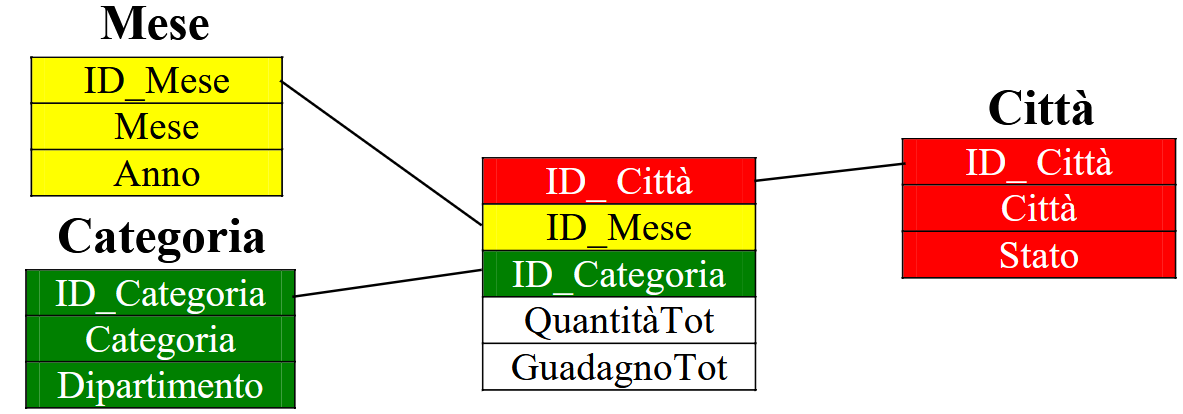
\includegraphics[width=0.7\textwidth]{capitoli/05_Data warehouse_progettazione fisica e alimentazione/images/def_vista_v3}
    \caption{Definizione SQL di una vista materializzata.}
    \label{fig:def-vista-v3}
\end{figure}

\noindent\textbf{Avvertenza sulle metriche:} Una singola vista materializzata può essere utilizzata per rispondere a più interrogazioni diverse, aggregando ulteriormente i dati precalcolati. Tuttavia, bisogna prestare estrema attenzione all'operatore di aggregazione. Ad esempio, non è possibile calcolare la media delle medie. Le metriche memorizzate nella vista devono permettere il calcolo corretto ai livelli di dettaglio superiori (ad esempio, memorizzando somma e conteggio anziché direttamente la media).

\subsubsection{Il Reticolo Multidimensionale}
Per visualizzare le possibili aggregazioni e le dipendenze tra di esse, si utilizza il \textbf{reticolo multidimensionale} (o reticolo delle viste). Ogni nodo del reticolo rappresenta una possibile granularità (una combinazione di attributi dimensionali). 

Il nodo di partenza (spesso in basso) rappresenta il dettaglio massimo presente nella tabella dei fatti (es. Prodotto, Data, Negozio). Risalendo le gerarchie delle dimensioni, si ottengono viste via via più aggregate (es. Categoria, Mese, Città).
Se esiste un collegamento diretto (un arco) tra un nodo $A$ e un nodo $B$ posizionato più in alto, significa che il risultato della vista $A$ può essere utilizzato per calcolare il risultato della vista $B$. 

% FIGURA ORIGINALE DA RECUPERARE DALLE SLIDE
% Slide di provenienza: Reticolo multidimensionale
% Tipo: Grafo/Schema concettuale
% Descrizione: Reticolo che mostra i nodi delle viste (V2, V3, V4, ecc.) e i collegamenti tra le aggregazioni possibili.
% Punto di inserimento: Qui, per illustrare le dipendenze tra i livelli di raggruppamento.
% File da inserire: reticolo_viste
\begin{figure}[H]
    \centering
    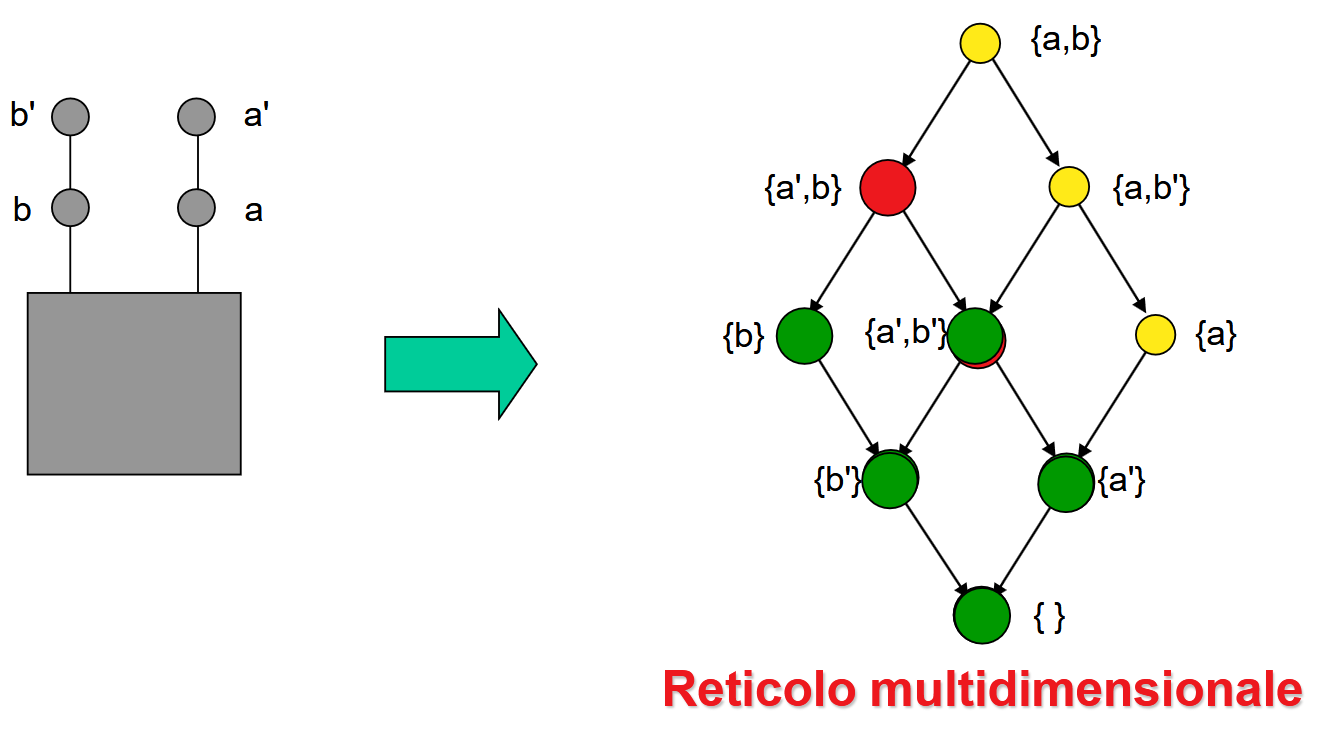
\includegraphics[width=0.85\textwidth]{capitoli/05_Data warehouse_progettazione fisica e alimentazione/images/reticolo_viste}
    \caption{Esempio di reticolo multidimensionale che illustra le dipendenze tra le viste materializzabili.}
    \label{fig:reticolo-viste}
\end{figure}

\noindent\textbf{L'importanza delle Gerarchie:}
Durante la lezione, il professore ha sottolineato un errore concettuale comune nella lettura del reticolo. Affinché si possa aggregare da un livello a un altro (es. da Tipo Prodotto a Categoria, o da Città a Regione), deve esistere un vincolo gerarchico rigoroso. 
Ad esempio, dati come Data, Mese e Trimestre formano una gerarchia rigida. Al contrario, se Tipo e Categoria fossero dimensioni ortogonali (dove a un tipo non è associata una sola categoria univoca, come giorno della settimana e mese), non ci potrebbe essere un arco diretto nel reticolo. Il reticolo assume quindi validità solo se supportato dalla corretta definizione delle gerarchie dimensionali.

\subsubsection{Il Problema della Scelta delle Viste}
Il numero di possibili viste materializzabili in un Data Warehouse reale è enorme. Non è pensabile materializzarle tutte. La scelta costituisce un problema di ottimizzazione che mira a minimizzare specifiche funzioni di costo:
\begin{itemize}
    \item Il costo di esecuzione delle interrogazioni (che si abbassa aumentando le viste).
    \item Il costo di aggiornamento delle viste stesse (che si alza aumentando le viste, poiché a ogni refresh del data warehouse le viste vanno ricalcolate).
\end{itemize}
A ciò si aggiungono dei vincoli pratici:
\begin{itemize}
    \item Spazio su disco disponibile.
    \item Finestra temporale disponibile per l'aggiornamento notturno (se l'aggiornamento richiede 8 ore ma la finestra utile è di sole 4 ore, il sistema non è sostenibile).
\end{itemize}

% FIGURA ORIGINALE DA RECUPERARE DALLE SLIDE
% Slide di provenienza: Scelta delle viste (Sequenza di 4 slide)
% Tipo: Diagramma a barre/Grafico intuitivo
% Descrizione: Istogrammi che confrontano il tempo di esecuzione, il tempo di aggiornamento e lo spazio occupato tra tre soluzioni: una singola vista generale, tre viste specifiche, o una soluzione intermedia.
% Punto di inserimento: Qui, a supporto della spiegazione dei trade-off.
% File da inserire: grafici_scelta_viste
\begin{figure}[H]
    \centering
    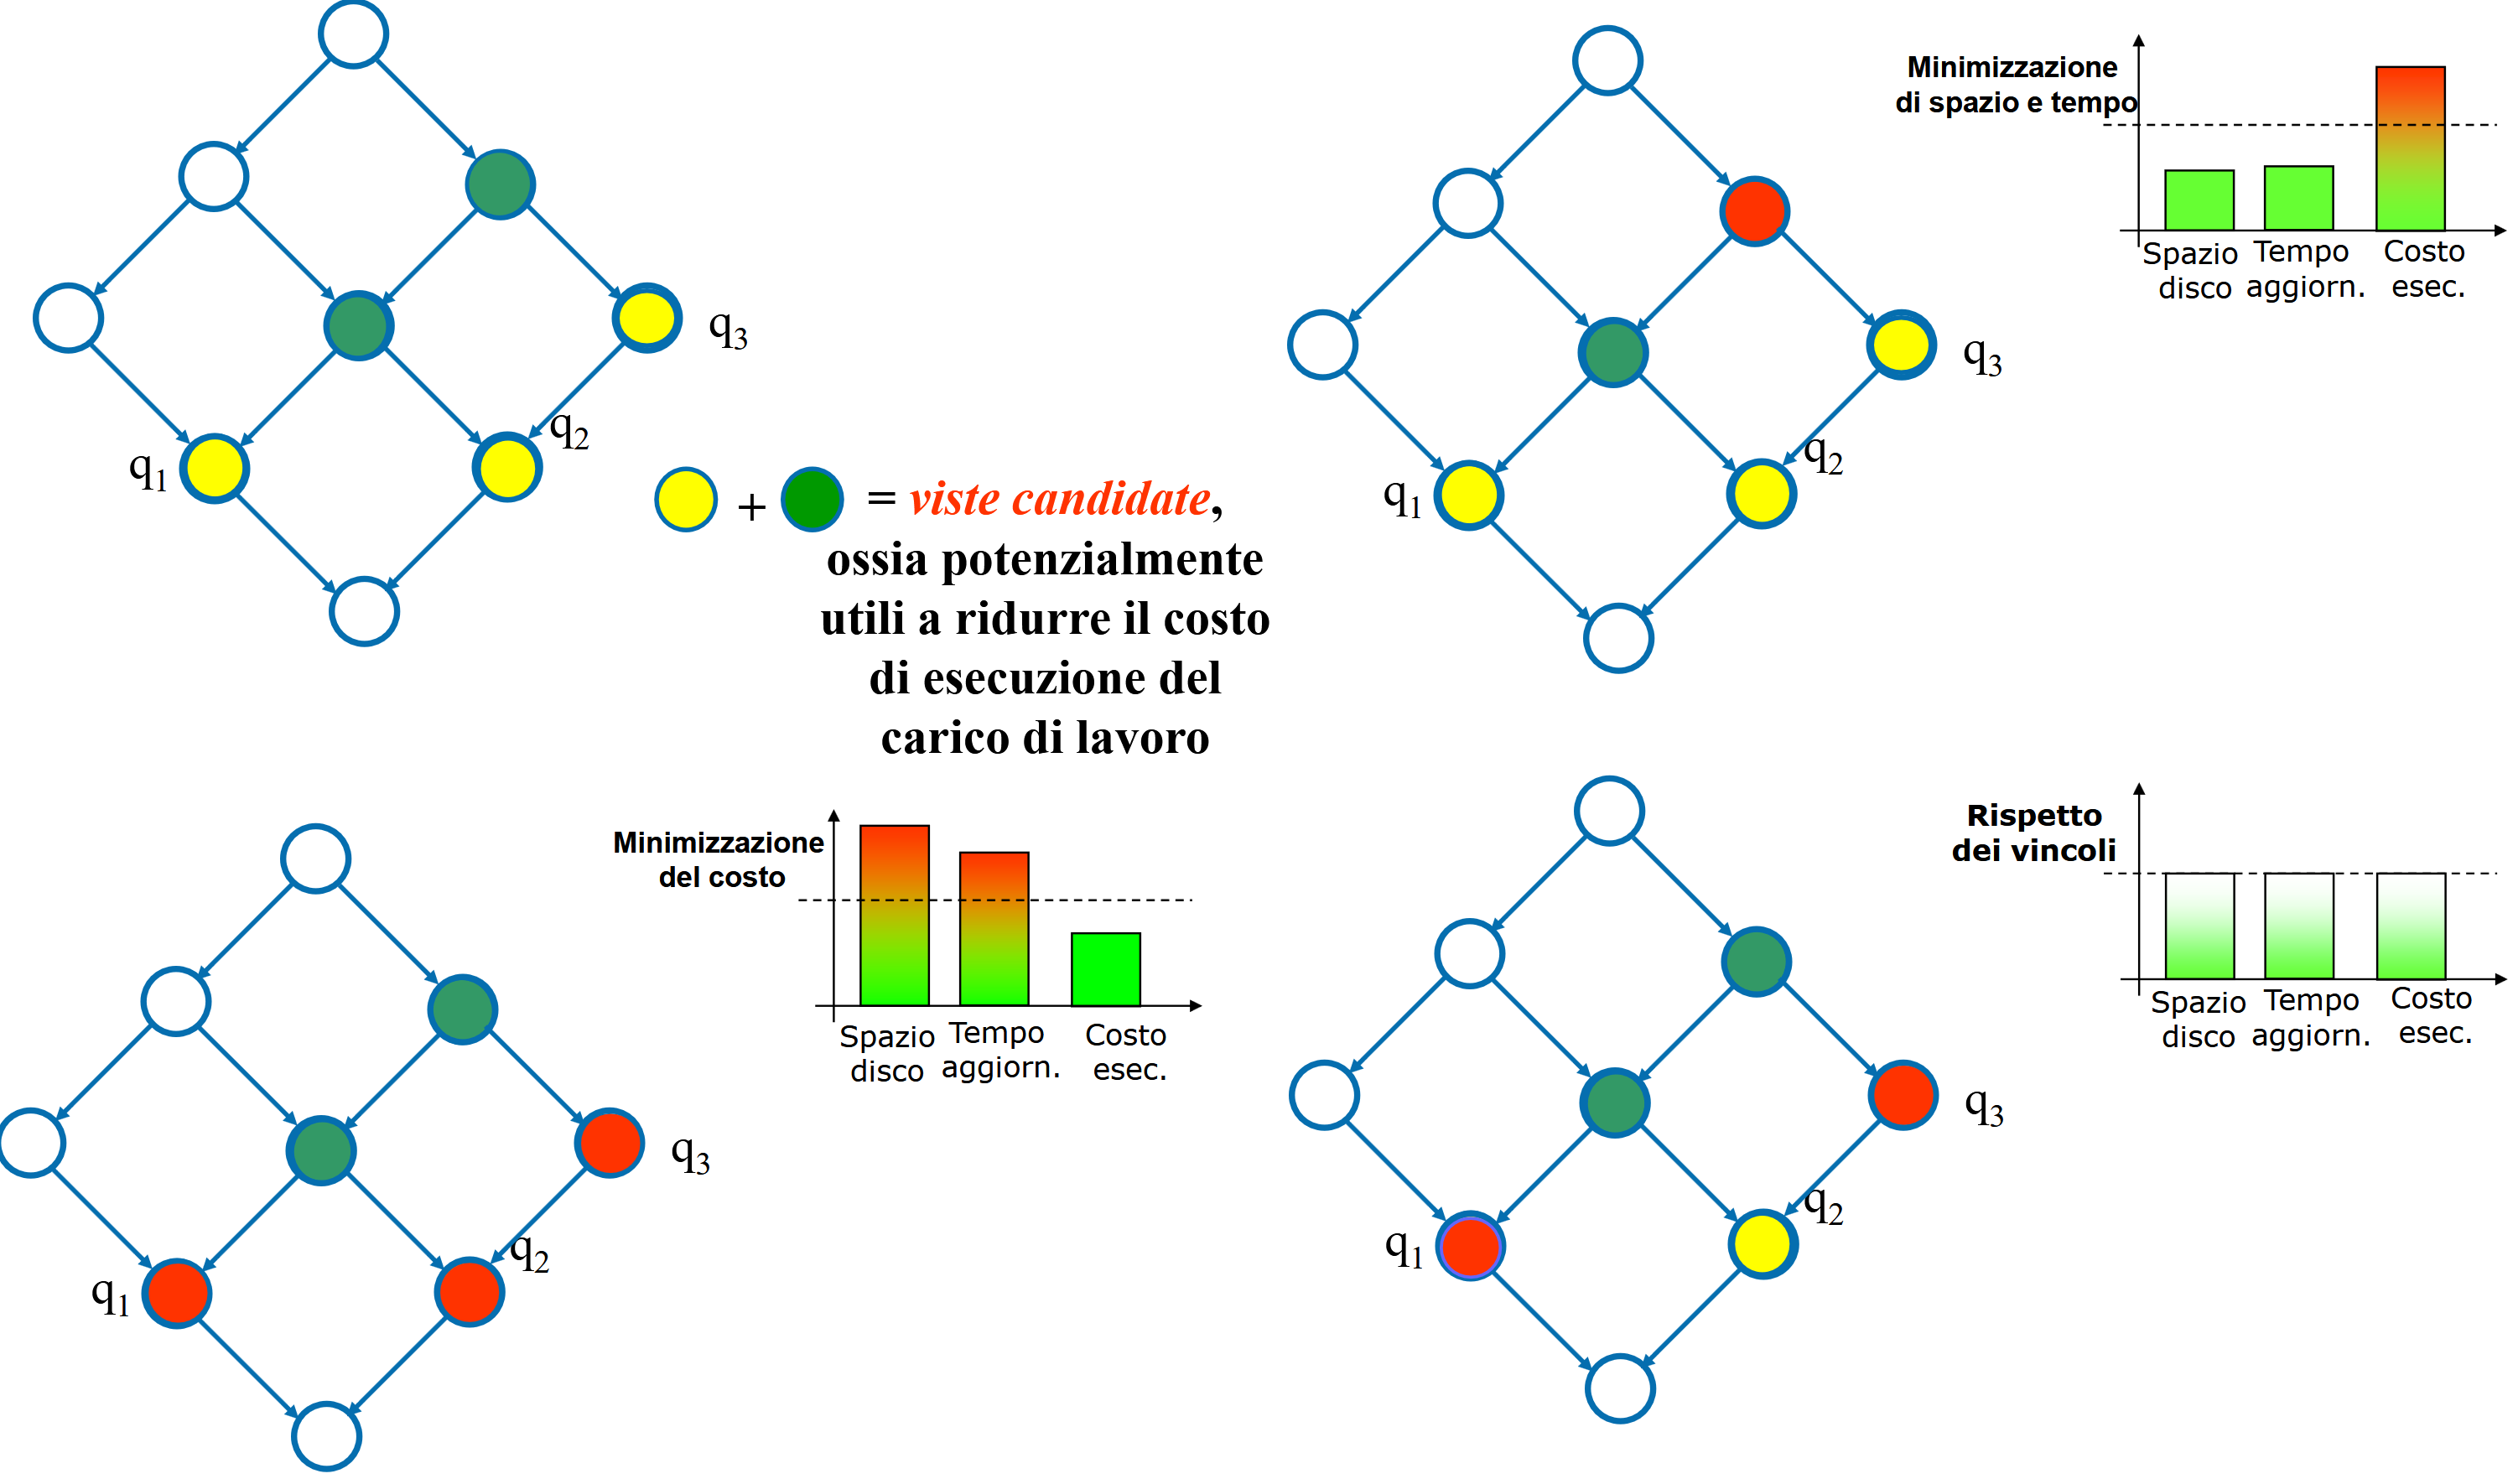
\includegraphics[width=0.9\textwidth]{capitoli/05_Data warehouse_progettazione fisica e alimentazione/images/grafici_scelta_viste}
    \caption{Analisi dei costi per la scelta delle viste ottimali: bilanciamento tra spazio, tempo di aggiornamento e tempo di query.}
    \label{fig:scelta-viste-costi}
\end{figure}

In sintesi, si può optare per tre strategie principali (illustrate nell'esempio discusso in aula per risolvere tre specifiche query):
\begin{enumerate}
    \item \textbf{Una sola vista aggregata molto specifica (basso livello):} Risponde a tutte le interrogazioni. Occupa più spazio e ha un tempo di esecuzione medio-alto per query molto aggregate, ma è l'unica vista da mantenere aggiornata.
    \item \textbf{Viste separate e mirate per ogni query:} Tempi di esecuzione minimi, ma massima occupazione di spazio e massimo costo di manutenzione/aggiornamento.
    \item \textbf{Soluzione intermedia:} Creare alcune viste intermedie nel reticolo che riescano a servire più query contemporaneamente offrendo il miglior compromesso tra tempo di risposta e costi di manutenzione.
\end{enumerate}

\subsection{Altre Strutture Fisiche: Indici e Parallelismo}
Oltre alle viste materializzate, la progettazione fisica si avvale di altre strutture:
\begin{itemize}
    \item \textbf{Indici B+-tree:} Poco adatti per gli attributi dimensionali del data warehouse che spesso hanno una cardinalità bassa (es. sesso, stato civile, regione).
    \item \textbf{Indici Bitmap e Indici di Join:} Strutture più efficienti per gli attributi dimensionali, frequentemente coinvolti nei predicati di selezione e nelle operazioni di join.
\end{itemize}
Il \textbf{tuning} del database è la fase operativa in cui, tramite il monitoraggio, si verifica se l'ottimizzatore sta effettivamente utilizzando gli indici e le viste creati dal progettista. In caso contrario, queste strutture fisiche consumano risorse (per l'aggiornamento) senza portare alcun beneficio e vanno rimosse o modificate.
Inoltre, le interrogazioni complesse (specialmente Join e Group By) beneficiano enormemente del \textbf{parallelismo} (frammentazione dei dati, e parallelizzazione inter-query e intra-query).

\section{Alimentazione del Data Warehouse (Processo ETL)}
L'architettura del Data Warehouse prevede che i dati di analisi siano fisicamente separati da quelli dei sistemi operazionali (sorgenti). Per mantenere aggiornato il Data Warehouse, è necessario un processo denominato \textbf{ETL} (Extraction, Transformation and Loading).
Spesso, tra le sorgenti e il data warehouse, si inserisce un'area di appoggio intermedia detta \textbf{Staging Area}, che porta l'architettura a tre livelli e facilita l'esecuzione di trasformazioni complesse.

Il processo ETL deve gestire due scenari ben distinti:
\begin{enumerate}
    \item \textbf{Il primo popolamento (tempo zero):} Il Data Warehouse e le dimensioni sono completamente vuoti e occorre acquisire una fotografia storica completa di tutto il periodo di interesse aziendale.
    \item \textbf{L'aggiornamento periodico (es. giornaliero):} Il Data Warehouse è già popolato, bisogna estrarre e caricare unicamente le variazioni e le nuove transazioni avvenute dall'ultimo caricamento.
\end{enumerate}

\subsection{Estrazione (Extraction)}
L'estrazione è la fase di acquisizione dei dati dalle sorgenti. Può essere:
\begin{itemize}
    \item \textbf{Statica:} Una vera e propria fotografia dell'intero database operazionale, eseguita per il primo popolamento.
    \item \textbf{Incrementale:} Si estraggono solo i dati inseriti, modificati o cancellati dall'ultimo aggiornamento.
\end{itemize}

\subsubsection{Le sfide dell'Estrazione Incrementale}
La complessità dell'estrazione incrementale dipende fortemente dalla natura dei dati operazionali:
\begin{itemize}
    \item \textbf{Dati storicizzati:} Il sistema OLTP salva storicamente tutte le variazioni (es. transazioni bancarie). L'estrazione è semplice perché ogni evento è tracciato.
    \item \textbf{Dati semi-storicizzati o Transitori:} Il DBMS mantiene solo l'immagine corrente del dato (es. scorte di magazzino in un dato istante) sovrascrivendo i valori precedenti. L'estrazione incrementale è molto complessa perché si perde traccia di cosa sia cambiato e di eventuali cancellazioni.
\end{itemize}

Per comprendere questa complessità, consideriamo il seguente esempio di estrazione incrementale tra il 4 aprile e il 6 aprile.

\begin{table}[H]
    \centering
    \caption{Fotografia DBMS al 4/4/2010}
    \begin{tabular}{cllc}
    \toprule
    \textbf{CodProdotto} & \textbf{Cliente} & \textbf{Qtà} \\
    \midrule
    1 & Greco di tufo & Malavasi & 50 \\
    2 & Barolo & Maio & 150 \\
    3 & Barbera & Lumini & 75 \\
    4 & Sangiovese & Cappelli & 45 \\
    \bottomrule
    \end{tabular}
\end{table}

\begin{table}[H]
    \centering
    \caption{Fotografia DBMS al 6/4/2010}
    \begin{tabular}{cllc}
    \toprule
    \textbf{Cod} & \textbf{Prodotto} & \textbf{Cliente} & \textbf{Qtà} \\
    \midrule
    1 & Greco di tufo & Malavasi & 50 \\
    2 & Barolo & Maio & 150 \\
    4 & Sangiovese & Cappelli & 145 \\
    5 & Vermentino & Maltoni & 25 \\
    6 & Trebbiano & Maltoni & 150 \\
    \bottomrule
    \end{tabular}
\end{table}

Un sistema ETL efficiente deve dedurre dalla differenza tra questi stati un file di aggiornamento che tracci esattamente le operazioni logiche avvenute, non potendosi limitare alle sole letture:

\begin{table}[H]
    \centering
    \caption{Estrazione Incrementale risultante (D=Delete, U=Update, I=Insert)}
    \begin{tabular}{cllcl}
    \toprule
    \textbf{Cod} & \textbf{Prodotto} & \textbf{Cliente} & \textbf{Qtà} & \textbf{Azione} \\
    \midrule
    3 & Barbera & Lumini & 75 & D (cancellato) \\
    4 & Sangiovese & Cappelli & 145 & U (modifica qtà da 45 a 145)\\
    5 & Vermentino & Maltoni & 25 & I (nuovo inserimento)\\
    6 & Trebbiano & Maltoni & 150 & I (nuovo inserimento)\\
    \bottomrule
    \end{tabular}
\end{table}

\subsubsection{Tecniche per l'estrazione incrementale}
Per realizzare concretamente questa estrazione, si possono utilizzare diverse tecniche, ognuna con precisi trade-off:

\begin{table}[H]
    \centering
    \resizebox{\textwidth}{!}{%
    \begin{tabular}{lccccc}
    \toprule
    & \textbf{Statica} & \textbf{Marche temp.} & \textbf{Assistita appl.} & \textbf{Trigger} & \textbf{Log} \\
    \midrule
    Gestione dati transitori & NO & Incompleta & Completa & Completa & Completa \\
    Supporto sistemi a file & SI & SI & SI & SI & NO \\
    Complessità procedure & Bassa & Bassa & Alta & Media & Bassa \\
    Modifiche ad applicazioni& Nessuna & Probabile & Probabile & Nessuna & Nessuna \\
    Impatto prestazioni operaz.& Nessuna & Nessuna & Medio & Medio & Nessuna \\
    \bottomrule
    \end{tabular}%
    }
    \caption{Confronto semplificato tra le tecniche di estrazione (rielaborato dalle slide).}
    \label{tab:tecniche-estrazione}
\end{table}

\begin{itemize}
    \item \textbf{Assistita dall'applicazione:} L'applicativo stesso viene modificato per scrivere da qualche parte i dati che sta cambiando. Richiede modifiche ai programmi (applicazioni on top al DBMS) e aumenta il carico applicativo, ma è spesso l'unica via per i vecchi sistemi \textit{legacy}.
    \item \textbf{Uso del Log:} Si legge il file di log interno del DBMS (che per sua natura traccia ogni operazione per garantire la recovery). È molto efficiente e non impatta sul carico applicativo, ma il log è in formato proprietario del vendor del database.
    \item \textbf{Tramite Trigger:} Si programmano dei trigger interni al DBMS che scattano autonomamente su \texttt{INSERT}, \texttt{UPDATE} e \texttt{DELETE}. Non richiede la modifica del programma applicativo esterno, ma incrementa notevolmente il carico di lavoro del DBMS in fase transazionale.
    \item \textbf{Tramite Timestamp (Marche temporali):} Si aggiunge una colonna data/ora ai record per tracciare l'ultima modifica. È un metodo parziale perché fallisce nel tracciare i dati \textit{cancellati} (se il record scompare, scompare anche il suo timestamp).
\end{itemize}

\subsection{Pulitura (Data Cleansing)}
I dati estratti da sorgenti eterogenee presentano quasi sempre problemi di \textit{Data Quality}: duplicati, dati mancanti, formati non uniformi (es. "C.so" vs "Corso"), valori errati.
Le procedure di pulitura includono:
\begin{itemize}
    \item \textbf{Uso di dizionari:} Standardizzazione dei domini (es. unificare le sigle delle province, CAP validi).
    \item \textbf{Tecniche di fusione approssimata (Approximate Join e Purge/Merge):} Spesso uno stesso cliente è memorizzato in due filiali con grafie leggermente diverse (es. "Rossi M." e "Mario Rossi"). Non avendo una chiave univoca comune, bisogna applicare algoritmi di similarità testuale per identificare se si tratta della stessa entità e procedere all'unione dei record (purge/merge).
\end{itemize}

\noindent\textbf{Nota sull'Intelligenza Artificiale nell'ETL:}
Come sottolineato dal professore durante la lezione, i sistemi ETL moderni si stanno evolvendo rapidamente. Per affrontare problemi di pulitura complessa (come join approssimati senza chiavi certe o riconoscimento di entità), si sta diffondendo l'uso di tecniche di Data Science, inclusi algoritmi di clustering e l'uso di modelli linguistici di grandi dimensioni (LLM). L'ETL non è più solo una semplice procedura SQL, ma assomiglia sempre di più alla fase di \textit{data preparation} del Machine Learning.

% FIGURA ORIGINALE DA RECUPERARE DALLE SLIDE
% Slide di provenienza: Join approssimato / Purge/Merge / Esempio di pulitura
% Tipo: Esempi visivi e schemi
% Descrizione: Esempio di standardizzazione anagrafica (es. "Elena Baralis C.so Duca...") e schema del join approssimato.
% Punto di inserimento: Qui, a corredo della spiegazione del cleansing.
% File da inserire: schemi_pulitura
\begin{figure}[H]
    \centering
    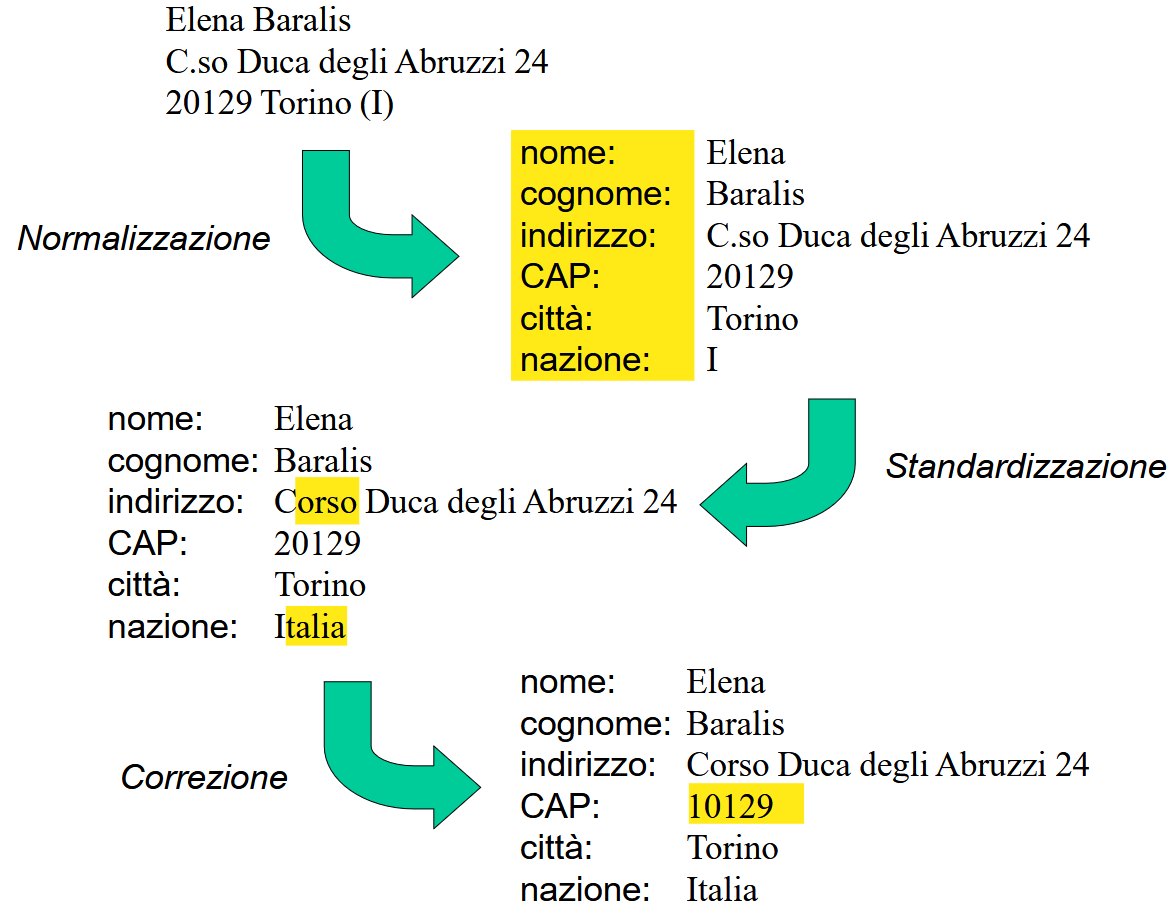
\includegraphics[width=0.75\textwidth]{capitoli/05_Data warehouse_progettazione fisica e alimentazione/images/schemi_pulitura}
    \caption{Esempi operativi di pulitura e risoluzione del problema del Purge/Merge.}
    \label{fig:schemi-pulitura}
\end{figure}

\subsection{Trasformazione}
Questa fase converte i dati dal formato in cui sono memorizzati operazionalmente a quello integrato del data warehouse. Questo passaggio, che di norma si completa nella Staging Area, prevede:
\begin{itemize}
    \item Passaggio allo \textbf{schema riconciliato} (notazione uniforme).
    \item Generazione dei \textbf{valori aggregati} se richiesti dallo schema.
    \item \textbf{Generazione delle chiavi surrogate:} Fondamentale per svincolare l'identificativo interno del data warehouse dalle chiavi applicative (che potrebbero cambiare nel tempo nei sistemi sorgente o presentare conflitti).
\end{itemize}

\subsection{Caricamento (Loading)}
La fase finale è la propagazione dei dati trasformati fisicamente nel Data Warehouse. 
Esiste una \textbf{gerarchia rigorosa e obbligatoria} per l'ordine di caricamento, al fine di rispettare l'integrità referenziale. I passi sono i seguenti:
\begin{enumerate}
    \item \textbf{Alimentazione delle Dimensioni:} Prima di poter caricare un evento, le entità che lo descrivono devono esistere. 
    Il sistema legge gli aggiornamenti dalla Staging Area, verifica se il record dimensionale esiste già (es. un cliente). Se esiste, ne estrae la \textit{chiave surrogata}; se non esiste, inserisce il nuovo record generando una nuova chiave.
    \item \textbf{Alimentazione della Fact Table:} I nuovi eventi vengono inseriti nella tabella dei fatti. Durante questo inserimento, il sistema non usa i codici operazionali originali, ma recupera (tramite query) le \textit{chiavi surrogate} che sono state appena aggiornate/generate nel passo 1.
    \item \textbf{Aggiornamento delle Viste Materializzate e degli Indici:} Poiché i dati di base sono cambiati, tutte le strutture fisiche di supporto (che contengono aggregazioni precalcolate) devono essere riallineate con i nuovi valori.
\end{enumerate}

% FIGURA ORIGINALE DA RECUPERARE DALLE SLIDE
% Slide di provenienza: Alimentazione delle dimensioni / Alimentazione delle fact table
% Tipo: Diagramma di flusso
% Descrizione: Diagrammi di flusso che mostrano la logica di inserimento dei dati nelle dimensioni (verifica esistenza -> insert/select) e l'inserimento nella fact table tramite lookup delle chiavi surrogate.
% Punto di inserimento: Qui, a chiusura del capitolo sull'ETL per mostrare visivamente la logica di caricamento.
% File da inserire: diagrammi_caricamento
\begin{figure}[H]
    \centering
    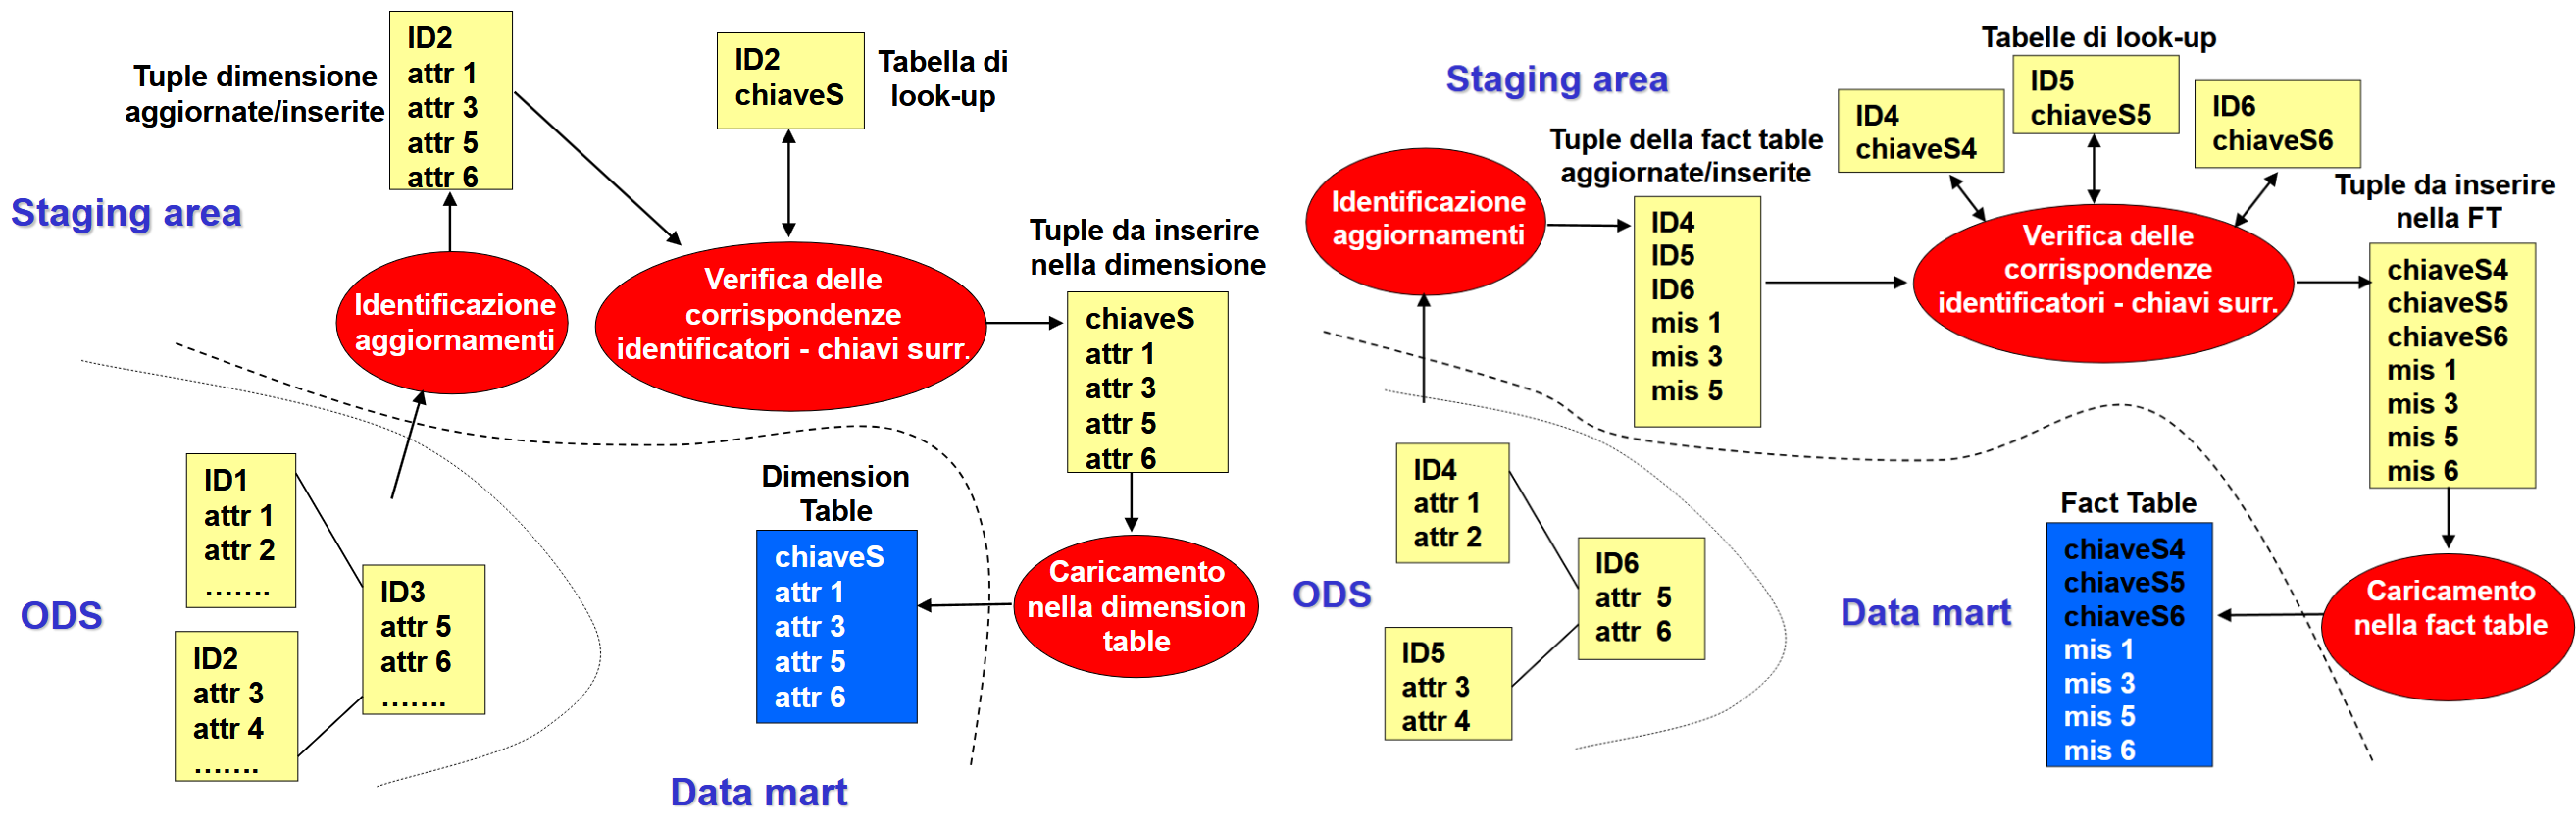
\includegraphics[width=1\textwidth]{capitoli/05_Data warehouse_progettazione fisica e alimentazione/images/diagrammi_caricamento}
    \caption{Flusso logico per l'alimentazione delle dimensioni e della fact table.}
    \label{fig:diagrammi-caricamento}
\end{figure}
\chapter{Estensioni al Linguaggio SQL in Oracle per l'Analisi dei Dati}

Questo capitolo introduce le estensioni al linguaggio SQL introdotte nel DBMS Oracle per supportare le operazioni di Business Intelligence e l'analisi dei dati in ambito Data Warehouse. Gran parte di queste estensioni si rifà allo standard SQL, pur presentando alcune specificità sintattiche, in particolare per quanto riguarda la definizione delle finestre di aggregazione.

Le funzionalità principali introdotte (funzioni OLAP) includono:
\begin{itemize}
    \item \textbf{Finestre di calcolo} (tramite la clausola \texttt{OVER} / \texttt{WINDOW});
    \item \textbf{Funzioni di ranking} per la generazione di classifiche (\texttt{RANK}, \texttt{DENSE\_RANK}, ecc.);
    \item \textbf{Estensione della clausola \texttt{GROUP BY}} (\texttt{ROLLUP}, \texttt{CUBE}, \texttt{GROUPING SETS}), che permette di generare raggruppamenti multipli con un singolo accesso ai dati.
\end{itemize}

\section{Le Finestre di Calcolo}

La finestra di calcolo permette di eseguire aggregazioni e analisi su un sottoinsieme di righe correlate alla riga corrente, senza collassare il risultato in un'unica riga per gruppo (come invece accade con la \texttt{GROUP BY} tradizionale). 
All'interno della finestra è possibile definire il partizionamento (\texttt{PARTITION BY}), l'ordinamento (\texttt{ORDER BY}) e l'ampiezza della finestra di aggregazione stessa.

Per illustrare il funzionamento della finestra di aggregazione, consideriamo una tabella relativa alle vendite con il seguente schema:
\texttt{VENDITE(Città, Data, Importo)}.

Nella definizione della porzione di finestra su cui effettuare il calcolo, è possibile adottare due approcci distinti: il raggruppamento a livello fisico e quello a livello logico.

\subsection{Raggruppamento a livello fisico (\texttt{ROWS})}

Il raggruppamento fisico conta esplicitamente il numero di tuple (righe) da includere nella finestra, a prescindere dal valore che assumono gli attributi. Questo approccio è utile quando si ha la garanzia che i dati siano continui, ma non tiene conto di eventuali "buchi" nella sequenza temporale o logica.

\paragraph{Esempio di raggruppamento fisico}
\textit{Selezionare, separatamente per ogni città, per ogni data l'importo e la media dell'importo considerando la riga corrente e le due righe che la precedono.}

In questo caso, calcoliamo una \textbf{media mobile}.
Prima di scrivere la query, analizziamo i passaggi logici:
\begin{enumerate}
    \item \textbf{Partizionamento}: I dati vanno calcolati "separatamente per ogni città", quindi occorre partizionare rispetto all'attributo \texttt{Città}.
    \item \textbf{Ordinamento}: È fondamentale ordinare i record per \texttt{Data}. Come sottolinea il professore, se non si effettuasse l'ordinamento, si rischierebbe di sommare una data di gennaio con una di dicembre, ottenendo un calcolo privo di senso logico.
    \item \textbf{Finestra}: Si richiede la riga corrente e le due \textit{precedenti}. Usando un approccio fisico parliamo esplicitamente di "righe", da cui la sintassi \texttt{ROWS BETWEEN 2 PRECEDING AND CURRENT ROW}.
\end{enumerate}

\begin{lstlisting}[language=SQL, basicstyle=\small\ttfamily, keywordstyle=\bfseries\color{blue}, frame=single]
SELECT Città, Data, Importo, 
       AVG(Importo) OVER (
           PARTITION BY Città
           ORDER BY Data
           ROWS BETWEEN 2 PRECEDING AND CURRENT ROW
       ) AS MediaMobile
FROM Vendite
ORDER BY Città, Data;
\end{lstlisting}
\textit{Nota:} Nella query manca l'operatore \texttt{GROUP BY} tradizionale. Sulla finestra applichiamo direttamente \texttt{AVG(Importo)}. L'\texttt{ORDER BY} finale, esterno alla funzione finestra, serve unicamente per una migliore visualizzazione dei risultati a schermo.

\subsection{Raggruppamento a livello logico (\texttt{RANGE})}

Il raggruppamento logico, a differenza di quello fisico, valuta il \textit{valore} assunto dal campo di ordinamento (tipicamente una data o un numero) per definire l'intervallo. Se, ad esempio, un negozio rimane chiuso in una specifica data, e quindi manca il record, l'approccio logico non andrà a ripescare un giorno ancora precedente per arrivare a "due righe", ma si limiterà a considerare i record effettivamente presenti nell'intervallo temporale richiesto.

\paragraph{Esempio di raggruppamento logico}
\textit{Selezionare, separatamente per ogni città, per ogni data l'importo e la media dell'importo considerando la riga corrente e le vendite avvenute nei due giorni precedenti.}

\begin{lstlisting}[language=SQL, basicstyle=\small\ttfamily, keywordstyle=\bfseries\color{blue}, frame=single]
SELECT Città, Data, Importo, 
       AVG(Importo) OVER (
           PARTITION BY Città
           ORDER BY Data
           RANGE BETWEEN INTERVAL '2' DAY PRECEDING AND CURRENT ROW
       ) AS MediaUltimi3Giorni
FROM Vendite
ORDER BY Città, Data;
\end{lstlisting}
La sintassi \texttt{RANGE BETWEEN INTERVAL '2' DAY PRECEDING AND CURRENT ROW} definisce un intervallo logico di tempo. Il professore precisa che, in Oracle, oltre a \texttt{DAY}, è possibile utilizzare anche \texttt{MONTH} e \texttt{YEAR}. L'inclusione di \texttt{CURRENT ROW} specifica che il calcolo della media comprende anche la riga corrente, valutando così gli ultimi 3 giorni complessivi (i 2 precedenti + quello attuale).

\section{Funzioni di Ranking}

Le funzioni di ranking permettono di associare ad ogni record una posizione all'interno di una classifica. Per i prossimi esempi, consideriamo il seguente schema relazionale che modella forniture aziendali:
\begin{itemize}
    \item \texttt{FRN(COD\_F, Nome, Sede\_F)}: Fornitori;
    \item \texttt{ART(COD\_A, Tipo, Colore, Peso)}: Articoli;
    \item \texttt{PRG(COD\_P, Nome, Sede\_P)}: Progetti;
    \item \texttt{FAP(COD\_F, COD\_P, COD\_A, Q)}: Quantità \texttt{Q} di articolo fornita per un progetto da un fornitore.
\end{itemize}

\subsection{\texttt{RANK} e \texttt{DENSE\_RANK}}

\paragraph{Esempio: Classifica di vendita degli articoli}
\textit{Selezionare per ogni articolo la quantità totale fornita e il ranking in funzione delle quantità totali fornite per ogni articolo.}

Poiché desideriamo una classifica generale di tutti gli articoli (i "top venduti"), non abbiamo bisogno di frammentare i dati: la finestra di calcolo \textbf{non richiederà un partizionamento}, ma soltanto un criterio di ordinamento.

\begin{lstlisting}[language=SQL, basicstyle=\small\ttfamily, keywordstyle=\bfseries\color{blue}, frame=single]
SELECT COD_A, SUM(Q) AS QTot,
       RANK() OVER (
           ORDER BY SUM(Q)
       ) AS RankVendite
FROM FAP
GROUP BY COD_A;
\end{lstlisting}

\textbf{Osservazione sull'ordinamento:} Nel codice mostrato sulle slide, non è specificato \texttt{DESC} nell'\texttt{ORDER BY}. Il professore fa notare che un ordinamento naturale per una classifica di vendita sarebbe decrescente (il prodotto più venduto al primo posto). Tuttavia, non specificando nulla, il sistema ipotizza un ordinamento \textbf{ascendente} (\texttt{ASC}). Pertanto, il prodotto con la quantità minore otterrà la prima posizione.

La differenza fondamentale tra \texttt{RANK} e \texttt{DENSE\_RANK} risiede nella gestione dei \textbf{pari merito}:
\begin{itemize}
    \item \textbf{\texttt{RANK}}: a parità di valore assegna la stessa posizione, ma salta le posizioni successive (es. due record al 3° posto portano il record successivo al 5° posto).
    \item \textbf{\texttt{DENSE\_RANK}}: assegna la stessa posizione per i pari merito, ma \textit{non salta} le posizioni successive (es. due record al 3° posto, il successivo sarà al 4° posto).
\end{itemize}

\begin{table}[H]
\centering
\caption{Confronto dei risultati tra RANK() e DENSE\_RANK()}
\begin{tabular}{lrr | r}
\toprule
\textbf{COD\_A} & \textbf{QTot} & \textbf{RankVendite (RANK)} & \textbf{DenseRankVendite (DENSE\_RANK)} \\
\midrule
A2 & 300  & 1 & 1 \\
A5 & 1100 & 2 & 2 \\
A4 & 1300 & 3 & 3 \\
A6 & 1300 & 3 & 3 \\
A1 & 1900 & 5 & 4 \\
A3 & 4500 & 6 & 5 \\
\bottomrule
\end{tabular}
\end{table}

\subsection{Doppio Ranking}

È possibile definire all'interno della medesima \texttt{SELECT} molteplici colonne di rank, calcolate rispetto a criteri di ordinamento differenti. Questo avviene perché la funzione genera semplicemente una nuova colonna aggiuntiva rispetto ai dati esistenti.

\paragraph{Esempio di doppio ranking}
\textit{Selezionare per ogni articolo il codice, il peso, la quantità totale fornita, il ranking in funzione del peso e il ranking in funzione della quantità totale fornita.}

In questo caso, siccome vogliamo visualizzare anche il peso (attributo di \texttt{ART}) e calcolare la quantità (attributo di \texttt{FAP}), dobbiamo eseguire una \texttt{JOIN} tra le due tabelle.

\begin{lstlisting}[language=SQL, basicstyle=\small\ttfamily, keywordstyle=\bfseries\color{blue}, frame=single]
SELECT ART.COD_A, ART.Peso,
       SUM(Q) AS QTot,
       RANK() OVER (ORDER BY ART.Peso) AS R_Peso,
       RANK() OVER (ORDER BY SUM(Q)) AS R_Vend
FROM FAP, ART
WHERE FAP.COD_A = ART.COD_A
GROUP BY ART.COD_A, ART.Peso
ORDER BY R_Peso;
\end{lstlisting}

\textbf{Osservazione sulla clausola \texttt{GROUP BY}:} L'attributo \texttt{Peso} è stato aggiunto alla \texttt{GROUP BY} poiché compare nella \texttt{SELECT} e non all'interno di una funzione di aggregazione. Tuttavia, come sottolineato a lezione, dato un articolo esiste uno e un solo peso associato; di conseguenza, l'aggiunta di questo attributo alla \texttt{GROUP BY} non altera in alcun modo la cardinalità o la semantica dei gruppi generati (si ha sempre un gruppo per ogni singolo prodotto).
Inoltre, è importante distinguere l'ordinamento per il ranking dal partizionamento: \textit{ranking in funzione del peso} significa che il peso fa da criterio di ordinamento (\texttt{ORDER BY ART.Peso} all'interno della clausola \texttt{OVER}), non di partizionamento. 

\begin{table}[H]
\centering
\caption{Risultato del doppio ranking}
\begin{tabular}{lrrrr}
\toprule
\textbf{COD\_A} & \textbf{Peso} & \textbf{Qtot} & \textbf{R\_Peso} & \textbf{R\_Vend} \\
\midrule
A1 & 12 & 1900 & 1 & 5 \\
A5 & 12 & 1100 & 1 & 2 \\
A4 & 14 & 1300 & 3 & 3 \\
A2 & 17 & 300  & 4 & 1 \\
A3 & 17 & 4500 & 4 & 6 \\
A6 & 19 & 1300 & 6 & 3 \\
\bottomrule
\end{tabular}
\end{table}

\subsection{Selezione Top-N nel Ranking (Utilizzo di Table Function)}

Spesso l'obiettivo aziendale non è analizzare un intero listino di 30.000 prodotti, ma restringere l'attenzione ai "Top N" (es. i 2 articoli più venduti) per evitare sprechi di risorse e migliorare la leggibilità.

Tuttavia, non è possibile filtrare direttamente il risultato di una funzione di rank inserendo una clausola del tipo \texttt{WHERE RankVendite <= 2} all'interno della stessa query. Il motivo, chiarito dal professore, risiede nell'\textbf{ordine di esecuzione delle istruzioni SQL}: la clausola \texttt{WHERE} valuta i record estratti prima della generazione delle colonne della \texttt{SELECT}, ma le funzioni finestra (come il rank) vengono processate proprio all'interno della \texttt{SELECT}.

La soluzione consiste nell'utilizzare le \textbf{Table Function} (o \textit{inline views}): una tabella temporanea generata localmente e a runtime, fornendo un'istruzione SQL come sorgente dati all'interno della clausola \texttt{FROM} della query principale.

\begin{lstlisting}[language=SQL, basicstyle=\small\ttfamily, keywordstyle=\bfseries\color{blue}, frame=single]
SELECT * FROM
  (
   SELECT COD_A, SUM(Q),
          RANK() OVER (ORDER BY SUM(Q)) AS RankVendite
   FROM FAP
   GROUP BY COD_A
  )
WHERE RankVendite <= 2;
\end{lstlisting}

Quando la query esterna elabora la clausola \texttt{FROM}, avvia l'esecuzione della sottointerrogazione. Questa genera una tabella virtuale provvista di tre colonne (tra cui \texttt{RankVendite}). A quel punto, la query esterna può regolarmente filtrare i dati applicando la \texttt{WHERE} sull'attributo precalcolato.

\section{Ulteriori Funzioni per Finestre di Calcolo}

Oltre alle tradizionali metriche di aggregazione e ai rank, Oracle rende disponibili ulteriori funzioni per caratterizzare e isolare i dati all'interno delle partizioni.

\subsection{\texttt{ROW\_NUMBER}}
La funzione \texttt{ROW\_NUMBER()} assegna un numero progressivo sequenziale ad ogni riga all'interno della partizione, basandosi sul criterio di ordinamento specificato.

\paragraph{Esempio}
\textit{Partizionare gli articoli in base alla tipologia ed enumerare in modo progressivo i dati all'interno di ogni partizione. All'interno di ogni partizione i dati sono ordinati in base al peso.}

\begin{lstlisting}[language=SQL, basicstyle=\small\ttfamily, keywordstyle=\bfseries\color{blue}, frame=single]
SELECT Tipo, Peso, 
       ROW_NUMBER() OVER (
           PARTITION BY Tipo
           ORDER BY Peso
       ) AS RowNumberPeso
FROM ART;
\end{lstlisting}

\textbf{Differenza tra \texttt{ROW\_NUMBER} e \texttt{RANK}}: 
L'aspetto più rilevante discusso in aula è il comportamento in caso di \textbf{pari merito}. A differenza di \texttt{RANK} e \texttt{DENSE\_RANK} (che assegnerebbero alle tuple con stesso peso il medesimo punteggio), \texttt{ROW\_NUMBER} non gestisce concettualmente i pari merito, ma forza un numero sequenziale. 
Se avessimo l'obiettivo di selezionare un numero esatto e fisso di elementi (es. i primi 5 prodotti), un filtro \texttt{<= 5} su un \texttt{RANK} in presenza di più pari merito potrebbe restituirci più di 5 righe in totale (es. tre prodotti a pari merito al 3° posto). Utilizzando \texttt{ROW\_NUMBER}, si garantisce l'estrazione di esattamente 5 record, operando una discriminazione arbitraria tra gli ex aequo all'interno del gruppo.

\subsection{\texttt{CUME\_DIST}}

La funzione \texttt{CUME\_DIST} calcola la \textbf{funzione cumulativa di distribuzione} dei valori all'interno di un gruppo (partizione).
Matematicamente, per ogni riga $x$, il valore di \texttt{CUME\_DIST} si ottiene come:
\[
\text{CUME\_DIST}(x) = \frac{\text{Numero di righe che precedono o hanno lo stesso valore di } x}{\text{Numero totale di righe nella partizione } (N)}
\]

\paragraph{Esempio esplicativo}
Prendendo come riferimento una singola partizione generata per gli articoli di tipo "Vite" (contenente $N=10$ tuple totali), ordinate per peso:
\begin{itemize}
    \item Se esiste $1$ solo record con peso 12, il suo \texttt{CUME\_DIST} sarà $1/10 = 0.1$ (ovvero, il 10\% dei record ha un peso minore o uguale a 12).
    \item Vi è $1$ record con peso 14. Cumulando il precedente si arriva alla seconda posizione: $2/10 = 0.2$.
    \item Vi sono \textbf{quattro} record a pari merito con peso 16. La funzione valuta tutti i valori minori \textbf{o uguali}, includendo di fatto tutto il blocco dei pari merito. La posizione massima di questo blocco è la sesta su dieci. Pertanto, ad \textit{ognuno} di questi 4 record verrà assegnato il valore $6/10 = 0.6$.
    \item I due record con peso 17 arrivano alla posizione 8 $\rightarrow$ $8/10 = 0.8$.
    \item L'ultimo record di peso 20 copre il 100\% della partizione $\rightarrow$ $10/10 = 1$.
\end{itemize}

Questa funzione risulta estremamente utile per studiare la distribuzione statistica di una determinata metrica all'interno di sottogruppi aziendali.

\subsection{\texttt{NTILE(n)}}

La funzione \texttt{NTILE(n)} viene utilizzata per suddividere i record di ogni partizione in $n$ sottogruppi (detti anche bucket). La funzione associa ad ogni record l'identificificativo del sottogruppo di appartenenza.

Oracle cerca di distribuire il numero di tuple in maniera omogenea. Se il numero totale di righe non è perfettamente divisibile per $n$, le dimensioni dei bucket avranno cardinalità il più possibile uniformi (con tolleranza $\pm 1$).

\paragraph{Esempio}
\textit{Partizionare in base alla tipologia, ordinare in base al peso, e suddividere in 3 sottogruppi.}
\begin{lstlisting}[language=SQL, basicstyle=\small\ttfamily, keywordstyle=\bfseries\color{blue}, frame=single]
SELECT Tipo, Peso, 
       NTILE(3) OVER (
           PARTITION BY Tipo
           ORDER BY Peso
       ) AS Ntile3Peso
FROM ART;
\end{lstlisting}

Riprendendo la partizione "Vite" di $N=10$ tuple, per suddividerla in 3 gruppi occorrono dimensioni che, sommate, diano 10. Il motore SQL allocherà i primi 4 record al gruppo 1, i successivi 3 al gruppo 2 e gli ultimi 3 al gruppo 3. Ad ogni record viene assegnato l'identificativo 1, 2 o 3, permettendo facilmente selezioni basate su fasce (ad esempio, isolare il "terzo medio" dei dati). Se una partizione possiede meno tuple del valore $n$ (es. partizione "Barra" ha un solo record), verrà generato solamente il sottogruppo 1.
\chapter{Data Lakes}


\chapter{Data Mining Process}


\chapter{Data Preparation}


\chapter{Data Mining: Association Rules}


\chapter{Data Mining: Classificazione}


\chapter{Data Mining: Clustering}




\chapter{ESERCIZI}
\chapter{Interrogazioni Analitiche in SQL Esteso: Esercitazione Pratica}

Questo capitolo è dedicato allo svolgimento di una serie di interrogazioni analitiche utilizzando le estensioni di SQL (come quelle supportate da Oracle), con particolare attenzione all'utilizzo delle funzioni di finestra (\textit{window functions}) per il calcolo di ranking e incassi cumulativi.

\section{Osservazione preliminare: Ordinamento e selezione degli ultimi elementi}
Prima di affrontare l'esercitazione sul Data Warehouse, è utile fare una considerazione tecnica emersa durante la lezione riguardo alla selezione degli ultimi elementi di una classifica (ad esempio, gli ultimi 10 elementi). 

Un approccio per ottenere questo risultato consiste nell'ordinare i dati in modo inverso rispetto al criterio logico della classifica (ad esempio, se la classifica normalmente è decrescente, si ordinano i dati in modo crescente, o viceversa) e successivamente estrarre i primi 10 record. Dal punto di vista del motore di ricerca e del recupero del dato, questo metodo è molto efficiente e corretto. Tuttavia, bisogna prestare attenzione alla \textbf{visualizzazione}: estraendo i record con un ordinamento inverso, l'elenco risulterà capovolto (es. l'elemento in decima posizione apparirà per primo, seguito dal nono, dall'ottavo, e così via). 

La logica di recupero dei dati è quindi separata dalla logica di visualizzazione. Se c'è la necessità di conoscere la posizione assoluta (il \textit{rank} esatto) di quegli elementi all'interno della totalità dei dati, sarà necessario effettuare un calcolo aggiuntivo sul numero totale dei record (o sui valori distinti assunti dall'attributo di ranking).

\section{Analisi dello Schema del Data Warehouse}
Le interrogazioni che andremo a risolvere si basano su uno schema di Data Warehouse strutturato secondo il Dimensional Fact Model. Lo schema è composto da una tabella dei fatti centrale e da quattro dimensioni.

Le tabelle a disposizione sono le seguenti:
\begin{itemize}
    \item \textbf{Cliente} (\texttt{CodCliente}, \texttt{Cliente}, \texttt{Provincia}, \texttt{Regione})
    \item \textbf{Categoria} (\texttt{CodCat}, \texttt{Categoria})
    \item \textbf{Agente} (\texttt{CodAgente}, \texttt{Agente}, \texttt{Agenzia})
    \item \textbf{Tempo} (\texttt{CodTempo}, \texttt{Mese}, \texttt{Trimestre}, \texttt{Semestre}, \texttt{Anno})
    \item \textbf{Fatturato} (\texttt{CodTempo}, \texttt{CodCliente}, \texttt{CodCatArticolo}, \texttt{CodAgente}, \texttt{TotFatturato}, \texttt{NumArticoli}, \texttt{TotSconto})
\end{itemize}

\subsection{Gerarchie e particolarità delle Dimensioni}
È fondamentale analizzare le gerarchie presenti all'interno delle dimensioni prima di procedere con le interrogazioni:
\begin{itemize}
    \item \textbf{Dimensione Cliente:} Presenta la gerarchia canonica in cui a ogni cliente è associata una sola provincia, e ogni provincia appartiene a una sola regione.
    \item \textbf{Dimensione Tempo:} Segue una gerarchia rigida in cui dato un mese esiste un solo trimestre, che a sua volta è collegato univocamente a un semestre e, infine, all'anno.
    \item \textbf{Dimensione Agente:} Ogni agente è associato a una e una sola agenzia, mentre la stessa agenzia gestisce più agenti.
    \item \textbf{Dimensione Categoria:} Questa tabella possiede un solo attributo descrittivo (\texttt{Categoria}) oltre alla chiave. Nella teoria del Data Warehousing, una dimensione con un solo attributo viene definita \textbf{dimensione degenere} (\textit{Junk Dimension}). Tuttavia, in questo schema è stata modellata come una tabella dimensionale tradizionale: questa scelta progettuale è giustificata dall'ipotesi che, in futuro, si possano aggiungere nuovi attributi o creare nuove gerarchie associate alla categoria.
\end{itemize}

La tabella dei fatti \textbf{Fatturato} ha una chiave primaria composta dai codici delle quattro dimensioni (\texttt{CodTempo}, \texttt{CodCliente}, \texttt{CodCatArticolo}, \texttt{CodAgente}). Le \textbf{metriche} su cui possiamo eseguire i calcoli sono tre: il totale del fatturato (\texttt{TotFatturato}), il numero degli articoli venduti (\texttt{NumArticoli}) e il totale dello sconto (\texttt{TotSconto}).

% ==========================================
% ESERCIZIO 1
% ==========================================
\section{Esercizio 1: Calcolo di aggregati e Ranking Globale}

\subsection{Testo della richiesta}
Visualizzare per ogni categoria di articoli:
\begin{enumerate}
    \item la categoria;
    \item la quantità totale fatturata per la categoria in esame;
    \item il fatturato totale associato alla categoria in esame;
    \item il rank della categoria in funzione della quantità totale fatturata;
    \item il rank della categoria in funzione del fatturato totale.
\end{enumerate}

\subsection{Ragionamento e Passaggi Logici}
Per rispondere alla query, dobbiamo incrociare i dati tra la tabella dei fatti \texttt{Fatturato} e la dimensione \texttt{Categoria}. La condizione di join sarà \texttt{Fatturato.CodCatArticolo = Categoria.CodCat}.

Poiché la richiesta richiede dati aggregati "per ogni categoria", è necessario applicare un'operazione di raggruppamento (\texttt{GROUP BY Categoria}). Le metriche base sono facilmente ricavabili applicando la funzione \texttt{SUM()} agli attributi \texttt{NumArticoli} (per la quantità totale) e \texttt{TotFatturato}.

Il calcolo del \textit{rank} richiede l'utilizzo delle funzioni di finestra (\texttt{RANK() OVER}). 
È importante chiederci se sia necessario partizionare i dati. In questo specifico caso, \textbf{non serve il partizionamento} (\texttt{PARTITION BY}). Il motivo risiede nel fatto che la query base genera un singolo record per ogni categoria. Pertanto, noi vogliamo assegnare una posizione in classifica a ciascuna categoria calcolata rispetto a \textit{tutte} le altre. Non essendoci un livello gerarchico superiore a "categoria" nel nostro schema rispetto al quale calcolare classifiche separate, la finestra di calcolo si applica all'intero set di dati raggruppato.

Viene richiesto di calcolare il rank due volte, con due criteri di ordinamento diversi:
\begin{itemize}
    \item \texttt{ORDER BY SUM(NumArticoli) DESC}: per assegnare la prima posizione alla categoria con la maggiore quantità di articoli venduti. L'uso di \texttt{DESC} assicura che il valore più alto abbia rank 1.
    \item \texttt{ORDER BY SUM(TotFatturato) DESC}: per calcolare la classifica in base al ricavo.
\end{itemize}

\subsection{Codice SQL}
\begin{lstlisting}[language=SQL, basicstyle=\ttfamily\small, keywordstyle=\color{blue}, stringstyle=\color{red}, commentstyle=\color{green!60!black}]
SELECT 
    C.Categoria,
    SUM(F.NumArticoli) AS QuantitaTotale,
    SUM(F.TotFatturato) AS FatturatoTotale,
    RANK() OVER (
        ORDER BY SUM(F.NumArticoli) DESC
    ) AS RankPerQuantita,
    RANK() OVER (
        ORDER BY SUM(F.TotFatturato) DESC
    ) AS RankPerFatturato
FROM 
    Fatturato F, 
    Categoria C
WHERE 
    F.CodCatArticolo = C.CodCat
GROUP BY 
    C.Categoria;
\end{lstlisting}

% ==========================================
% ESERCIZIO 2
% ==========================================
\section{Esercizio 2: Ranking con Partizionamento}

\subsection{Testo della richiesta}
Visualizzare per ogni provincia:
\begin{enumerate}
    \item la provincia;
    \item la regione della provincia;
    \item il fatturato totale associato alla provincia;
    \item il rank della provincia in funzione del fatturato totale, separato per regione.
\end{enumerate}

\subsection{Ragionamento e Passaggi Logici}
Le informazioni geografiche (Provincia e Regione) si trovano nella dimensione \texttt{Cliente}. Bisognerà quindi effettuare un join tra \texttt{Fatturato} e \texttt{Cliente} tramite l'attributo \texttt{CodCliente}.

La query richiede di considerare l'aggregazione a livello di provincia. È necessario usare la clausola \texttt{GROUP BY Provincia}. 
Sorge spontanea una domanda: possiamo inserire anche la \texttt{Regione} nella clausola \texttt{SELECT} e nel \texttt{GROUP BY}? La risposta è \textbf{sì}. Data una provincia, esiste infatti una e una sola regione di appartenenza (relazione funzionale $N:1$). Inserire \texttt{Regione} nel \texttt{GROUP BY} non altera la granularità del risultato (che rimane a livello di provincia), ma permette di proiettare la regione nella selezione.

\paragraph{Il concetto semantico del Rank rispetto al raggruppamento:}
Durante la lezione il professore ha precisato un dettaglio semantico. Quando eseguiamo un \texttt{GROUP BY} su un singolo attributo (es. solo per provincia), possiamo dire di "assegnare il rank all'attributo Provincia". Quando però raggruppiamo per più attributi congiuntamente, l'espressione più formalmente corretta è "assegnare un rank ad ogni record generato dalla query", poiché la riga rappresenta la combinazione degli attributi raggruppati.

Il calcolo del rank in questo esercizio introduce la clausola \texttt{PARTITION BY}. Viene esplicitamente richiesto che il rank sia "separato per regione". Ciò significa che per ogni regione si aprirà una nuova finestra di calcolo, e all'interno di quella regione la provincia con il fatturato più alto assumerà rank 1.

\subsection{Codice SQL}
\begin{lstlisting}[language=SQL, basicstyle=\ttfamily\small, keywordstyle=\color{blue}, stringstyle=\color{red}, commentstyle=\color{green!60!black}]
SELECT 
    C.Provincia,
    C.Regione,
    SUM(F.TotFatturato) AS FatturatoTotale,
    RANK() OVER (
        PARTITION BY C.Regione
        ORDER BY SUM(F.TotFatturato) DESC
    ) AS RankProvinciaPerRegione
FROM 
    Fatturato F, 
    Cliente C
WHERE 
    C.CodCliente = F.CodCliente
GROUP BY 
    C.Provincia, 
    C.Regione;
\end{lstlisting}

% ==========================================
% ESERCIZIO 3
% ==========================================
\section{Esercizio 3: Ranking Multi-Dimensionale}

\subsection{Testo della richiesta}
Visualizzare per ogni provincia e mese:
\begin{enumerate}
    \item la provincia;
    \item la regione della provincia;
    \item il mese;
    \item il fatturato totale associato alla provincia nel mese in esame;
    \item il rank della provincia in funzione del fatturato totale, separato per mese.
\end{enumerate}

\subsection{Ragionamento e Passaggi Logici}
Questa query estende la precedente aggiungendo la dimensione temporale. L'interrogazione richiederà di unire tre tabelle: \texttt{Fatturato}, \texttt{Cliente} e \texttt{Tempo}.

Le entità fondamentali su cui basare il raggruppamento dettate dalla query sono \textbf{Provincia} e \textbf{Mese}. Come best-practice suggerita, quando si costruisce il raggruppamento, è utile inserire prima questi due attributi principali e aggiungere solo successivamente le eventuali dipendenze funzionali, come la \texttt{Regione}. Nonostante in SQL l'ordine degli attributi nel \texttt{GROUP BY} sia ininfluente sull'esecuzione, scriverli in questo modo aiuta lo sviluppatore ad avere ben chiara la granularità concettuale della query.

Il rank richiesto deve essere ricalcolato separatamente in ogni diverso periodo temporale. Di conseguenza, la finestra di calcolo deve essere definita indicando \texttt{PARTITION BY Mese}.

\subsection{Codice SQL}
\begin{lstlisting}[language=SQL, basicstyle=\ttfamily\small, keywordstyle=\color{blue}, stringstyle=\color{red}, commentstyle=\color{green!60!black}]
SELECT 
    C.Provincia,
    T.Mese,
    C.Regione,
    SUM(F.TotFatturato) AS FatturatoTotale,
    RANK() OVER (
        PARTITION BY T.Mese
        ORDER BY SUM(F.TotFatturato) DESC
    ) AS RankProvinciaPerMese
FROM 
    Fatturato F, 
    Cliente C, 
    Tempo T
WHERE 
    C.CodCliente = F.CodCliente 
    AND F.CodTempo = T.CodTempo
GROUP BY 
    C.Provincia, 
    T.Mese, 
    C.Regione;
\end{lstlisting}

% ==========================================
% ESERCIZIO 4
% ==========================================
\section{Esercizio 4: Calcolo dell'Incasso Cumulativo (Running Total)}

\subsection{Testo della richiesta}
Visualizzare per ogni regione e mese:
\begin{enumerate}
    \item la regione;
    \item il mese;
    \item il fatturato totale associato alla regione nel mese in esame;
    \item l'incasso cumulativo al trascorrere dei mesi, separato per ogni regione;
    \item l'incasso cumulativo al trascorrere dei mesi, separato per ogni anno e regione.
\end{enumerate}

\subsection{Ragionamento e Passaggi Logici}
Questa interrogazione sposta il focus dalle classifiche alle \textbf{somme cumulative} nel tempo, che si realizzano combinando la funzione di aggregazione \texttt{SUM()} con una finestra basata sull'istruzione \texttt{ROWS UNBOUNDED PRECEDING}.

Per prima cosa, eseguiamo i join necessari (\texttt{Fatturato}, \texttt{Cliente}, \texttt{Tempo}) e definiamo la clausola \texttt{GROUP BY}. Gli attributi di raggruppamento principali sono \texttt{Regione} e \texttt{Mese}. Tuttavia, prestando attenzione all'ultima richiesta, notiamo che ci serve differenziare il calcolo cumulativo anche per \textbf{Anno}. Sappiamo che ogni \texttt{Mese} definisce univocamente un \texttt{Anno}; pertanto, dobbiamo obbligatoriamente aggiungere l'attributo \texttt{Anno} nel \texttt{GROUP BY} affinché esso diventi disponibile nella \texttt{SELECT} (e conseguentemente nella \texttt{PARTITION BY}).

Vediamo nel dettaglio i due incassi cumulativi richiesti:
\begin{itemize}
    \item \textbf{Incasso cumulativo separato per regione:}
    La formula richiede di sommare progressivamente i valori aggregati mensili. Si scrive \texttt{SUM(SUM(TotFatturato))}. Il partizionamento avviene solo rispetto a \texttt{Regione}. L'ordinamento, affinché l'accumulazione abbia senso cronologico, si effettua con \texttt{ORDER BY Mese}. Per sommare tutto dalla prima registrazione disponibile in quella partizione fino al mese corrente, si aggiunge la direttiva \texttt{ROWS UNBOUNDED PRECEDING}.
    
    \item \textbf{Incasso cumulativo separato per regione e per anno:}
    La logica è identica, ma in questo caso si richiede che all'inizio di ogni nuovo anno accertato il contatore "si azzeri". Per implementare questo comportamento, è sufficiente aggiungere l'attributo temporale alla partizione: \texttt{PARTITION BY Regione, Anno}. In questo modo, gennaio non sommerà i mesi dell'anno precedente, perché inizierà una nuova partizione.
\end{itemize}

\paragraph{Interpretazione fisica e temporale (Approfondimento in Lezione):}
Rispondendo alla perplessità di uno studente su come visualizzare mentalmente le due colonne generate in tempo reale, il professore ha fornito la seguente delucidazione. Supponiamo di avere un Data Warehouse popolato con i dati degli anni compresi tra il 2024 e il 2026:
\begin{itemize}
    \item La colonna del \textit{primo cumulativo} (solo per regione) presenterà un unico blocco che cresce costantemente per ogni regione. A Gennaio 2024 avremo l'incasso di un mese. A Febbraio 2024 la somma di due. Arrivando a Gennaio 2025, in questa colonna troveremo la somma di \textbf{tutti i 12 mesi del 2024 più Gennaio 2025}. 
    \item La colonna del \textit{secondo cumulativo} (regione e anno), invece, una volta raggiunto l'inizio del nuovo anno (Gennaio 2025), perderà memoria del 2024. Il suo valore coinciderà esclusivamente con l'incasso di Gennaio 2025 per poi riniziare ad accumulare fino a Dicembre 2025.
\end{itemize}
Infine, sui mesi futuri non conclusi o senza registrazioni (es. un presunto "Ottobre 2026" se non sono state effettuate vendite), i dati semplicemente non saranno generati, poiché il sistema lavora interrogando i record con granularità mensile fisicamente memorizzati nel Data Warehouse fino a quel momento.

\subsection{Codice SQL}
\begin{lstlisting}[language=SQL, basicstyle=\ttfamily\small, keywordstyle=\color{blue}, stringstyle=\color{red}, commentstyle=\color{green!60!black}]
SELECT 
    C.Regione,
    T.Anno,
    T.Mese,
    SUM(F.TotFatturato) AS FatturatoMese,
    SUM(SUM(F.TotFatturato)) OVER (
        PARTITION BY C.Regione
        ORDER BY T.Mese
        ROWS UNBOUNDED PRECEDING
    ) AS CumulativoStoricoPerRegione,
    SUM(SUM(F.TotFatturato)) OVER (
        PARTITION BY C.Regione, T.Anno
        ORDER BY T.Mese
        ROWS UNBOUNDED PRECEDING
    ) AS CumulativoAnnuoPerRegione
FROM 
    Fatturato F, 
    Cliente C, 
    Tempo T
WHERE 
    F.CodCliente = C.CodCliente
    AND F.CodTempo = T.CodTempo
GROUP BY 
    C.Regione, 
    T.Anno, 
    T.Mese;
\end{lstlisting}


\chapter{Progettazione di un Data Warehouse: Caso Studio Magazzini}

Il presente capitolo illustra il processo completo di progettazione di uno schema concettuale e logico per un Data Warehouse, partendo da un caso di studio aziendale. L'obiettivo didattico è applicare i concetti teorici per trasformare le specifiche di un committente in un modello dati ottimizzato per l'analisi (OLAP), partendo dall'ipotesi di avere a disposizione un database transazionale (OLTP) di origine da cui estrarre e aggregare le informazioni.

\section{Metodologia di Progettazione}

Prima di affrontare il caso di studio specifico, è fondamentale fissare i passi metodologici necessari per passare dalla richiesta del committente allo schema logico finale. La progettazione si articola nei seguenti punti:

\begin{enumerate}
    \item \textbf{Identificazione dei fatti di interesse e delle misure:} Un "fatto" rappresenta il nucleo dell'analisi aziendale. Le misure (o metriche) sono le grandezze numeriche che descrivono il fatto. Nel Data Warehouse, queste metriche sono solitamente espresse tramite operatori aggregabili (come somme o conteggi). Si evita, di norma, di memorizzare valori come le medie dirette, preferendo memorizzare numeratore e denominatore (es. totale e conteggio) poiché la media non è facilmente riaggregabile al variare della cardinalità.
    \item \textbf{Identificazione delle dimensioni e dei livelli minimi di aggregazione:} Le dimensioni rappresentano le prospettive (o assi) lungo le quali si vogliono "tagliare" o aggregare le metriche. Il livello minimo di aggregazione determina la granularità della tabella dei fatti (la \textit{fact table}): definisce il livello di dettaglio massimo a cui i dati saranno analizzabili.
    \item \textbf{Definizione delle gerarchie:} All'interno di ogni dimensione, gli attributi sono organizzati in gerarchie che rappresentano relazioni di tipo $1:N$ (ad esempio, una città appartiene a una sola provincia, ma una provincia contiene più città). Comprendere queste gerarchie è vitale per costruire correttamente i rami del nostro modello concettuale.
    \item \textbf{Costruzione dello schema concettuale:} Trasformazione dei requisiti in un modello grafico (es. \textit{Star Schema} o schema a stella), che evidenzia la fact table centrale e i rami dimensionali, gestendo casistiche particolari come relazioni molti-a-molti (gestite tramite doppi archi e tabelle ponte) o "dimensioni degeneri" (che non necessitano di una tabella dimensionale a sé stante).
    \item \textbf{Definizione dello schema logico:} Traduzione dello schema concettuale in tabelle relazionali, ponendo particolare attenzione alla formattazione degli attributi (specialmente quelli temporali) per far sì che le gerarchie, che si perdono nel passaggio allo schema logico, vengano implicitamente preservate all'interno dei dati.
    \item \textbf{Stima del carico di lavoro e verifica:} Controllo della validità del modello rispetto alle interrogazioni (\textit{query}) tipiche fornite dal committente, assicurandosi che il livello di aggregazione sia sufficiente per rispondere alle richieste senza essere inutilmente eccessivo.
\end{enumerate}

\section{Analisi delle Specifiche e Identificazione dei Fatti}

Il problema in esame riguarda una grande ditta italiana di elettrodomestici con magazzini distribuiti sul territorio nazionale. La dirigenza ha due necessità analitiche principali:
\begin{itemize}
    \item \textbf{Analisi dell'uso dei magazzini:} Capire la percentuale di utilizzo in funzione della dislocazione geografica per decidere su ampliamenti, ridimensionamenti o affitti a terzi.
    \item \textbf{Stima dei costi delle polizze assicurative:} Analizzare la copertura contro furti e danni, i cui premi si basano sulla quantità media giornaliera di prodotti presenti e sul loro valore complessivo, per le diverse categorie e modelli.
\end{itemize}

Leggendo le specifiche, emerge subito un'entità geografica di base: \textit{l'Italia}. Tuttavia, poiché tutti i magazzini si trovano in Italia, la Nazione rappresenta una \textbf{dimensione universo}. Mappare questa dimensione sarebbe ridondante: non faremmo mai aggregazioni per nazione in questo contesto, poiché il valore sarebbe sempre e solo "Italia". Pertanto, la scartiamo fin dall'inizio.

Sembra che ci troviamo di fronte a due fatti semanticamente distinti: l'occupazione fisica dello spazio e la valorizzazione dei prodotti per le assicurazioni. L'approccio più sicuro è modellarli inizialmente come due \textit{fact table} separate. Successivamente, se scoprissimo che condividono esattamente le stesse dimensioni allo stesso livello di granularità, potremmo valutarne l'unione per questioni di ottimizzazione; tuttavia, mantenerle separate all'inizio è la scelta metodologica corretta.

\section{Progettazione Concettuale: Schema a Stella}

\subsection{Fatto 1: Uso dei Magazzini}

Il primo fatto di interesse riguarda le superfici. Il testo specifica che l'azienda vuole analizzare "la percentuale giornaliera di superficie libera rispetto alla superficie totale disponibile".

\subsubsection{Identificazione delle Metriche}
Le misure da tracciare nella fact table sono due:
\begin{itemize}
    \item \textbf{Superficie libera:} È il dato che varia dinamicamente e descrive l'effettivo spazio vuoto.
    \item \textbf{Superficie totale disponibile:} Questo è un punto di attenzione cruciale. In molti casi, la capienza totale di un magazzino è un dato statico (o che varia molto raramente); se così fosse, sarebbe molto più efficiente modellarla come attributo della dimensione \textit{Magazzino}, risparmiando spazio (non la si traccerebbe ogni giorno per ogni magazzino). Tuttavia, le specifiche affermano esplicitamente: \textit{"La superficie totale disponibile per ogni magazzino può variare di giorno in giorno, in quanto alcune aree possono essere affittate a terzi o essere inagibili"}. Poiché varia giornalmente, \textbf{deve obbligatoriamente essere una metrica} tracciata giorno per giorno nella fact table.
\end{itemize}

\subsubsection{Identificazione delle Dimensioni e Gerarchie}
Le aggregazioni richieste per il Fatto 1 si basano su due dimensioni principali:

\textbf{1. Dimensione Spaziale (Luogo)} \\
L'analisi deve avvenire "in funzione del magazzino e del luogo in cui esso si trova (città, provincia, regione)".
Il livello minimo di aggregazione è chiaramente il \textbf{Magazzino}. Un magazzino non si divide su più città. La gerarchia è lineare (relazione $1:N$):
\[\text{Magazzino} \rightarrow \text{Città} \rightarrow \text{Provincia} \rightarrow \text{Regione}\]

\textbf{2. Dimensione Temporale} \\
L'analisi deve essere possibile a livello di singola \textbf{Data} (livello minimo), ma anche aggregabile per Mese, Trimestre, Quadrimestre, Semestre e Anno.
Costruire la gerarchia temporale richiede attenzione affinché ogni attributo mantenga una relazione univoca verso il livello superiore. Se indicassimo il "Mese" semplicemente con un numero da 1 a 12, non sapremmo a quale anno appartiene, rompendo la gerarchia logica in fase di traduzione tabellare.

Per preservare la gerarchia, i dati devono essere formattati includendo l'eredità del padre. Ad esempio:
\begin{itemize}
    \item Data: 12-10-2026
    \item Mese: 10-2026
    \item Trimestre: 3-2026 (indica il terzo trimestre dell'anno)
    \item Anno: 2026
\end{itemize}

La struttura gerarchica del tempo presenta alcune diramazioni dal Mese in poi:
\begin{itemize}
    \item \textbf{Dal Mese al Trimestre:} Esiste una relazione $1:N$ diretta (un mese appartiene a un solo trimestre).
    \item \textbf{Dal Mese al Quadrimestre:} Esiste una relazione $1:N$ diretta (un mese appartiene a un solo quadrimestre).
    \item \textbf{Tra Trimestre e Quadrimestre:} \textbf{Non esiste} alcuna gerarchia. Un quadrimestre non è formato da un numero intero di trimestri. Quindi Mese diverge in due rami separati.
    \item \textbf{Dal Trimestre al Semestre:} Due trimestri compongono esattamente un semestre, quindi esiste una freccia gerarchica tra Trimestre e Semestre.
    \item \textbf{Verso l'Anno:} Quadrimestre e Semestre convergono entrambi nell'Anno.
\end{itemize}

\textit{Osservazione aggiuntiva:} Come spiegato a lezione, si crea in questo modo un'abbondanza di dati ripetuti. In un database relazionale normale si ricaverebbe il mese dalla data per via programmatica. In un Data Warehouse questa ridondanza è voluta per accelerare le aggregazioni in lettura tramite indici. Inoltre, se fosse richiesto fare analisi comparative mensili prescindendo dall'anno (es. "Tutti gli incassi di ottobre di ogni anno"), sarebbe necessario aggiungere una dimensione "Mese dell'anno" (valori 1-12) collegata direttamente alla Data e non dipendente dall'Anno.

% FIGURA ORIGINALE DA RECUPERARE DALLE SLIDE
% Slide di provenienza: Da appunti lavagna virtuale della registrazione (costruzione Star Schema Fatto 1)
% Tipo: Schema concettuale a stella
% Descrizione: Diagramma con fact table centrale "Uso Magazzini" con metriche (superficie libera, superficie totale). Due rami dimensionali: Luogo (Magazzino -> Città -> Provincia -> Regione) e Tempo con le biforcazioni su Trimestre e Quadrimestre spiegate nel testo.
% Punto di inserimento: Qui
\begin{figure}[H]
    \centering
    % Sostituire il segnaposto con il percorso effettivo dell'immagine
    %\includegraphics[width=0.7\textwidth]{schema_fatto1_placeholder}
    \caption{Schema concettuale a stella per il fatto "Uso Magazzini", con evidenza della gerarchia temporale divergente.}
    \label{fig:star_schema_1}
\end{figure}


\subsection{Fatto 2: Stima dei Costi delle Polizze}

Il secondo obiettivo riguarda la valutazione del contenuto dei magazzini per scopi assicurativi.

\subsubsection{Identificazione delle Metriche}
I premi assicurativi sono calcolati considerando il numero di prodotti presenti e il loro valore complessivo.
Poiché l'analisi mira a descrivere queste quantità su base aggregata per tipologia e data, le metriche della \textit{fact table} saranno:
\begin{itemize}
    \item \textbf{Numero di prodotti:} Conteggio aggregato dei prodotti presenti nel magazzino in un determinato giorno, per un determinato modello.
    \item \textbf{Valore prodotti:} Il valore economico aggregato associato a tale quantità.
\end{itemize}
Il database OLTP di origine conterrà verosimilmente le tracce del singolo prodotto identificato dal suo numero di serie, ma in fase di estrazione verso il Data Warehouse aggregheremo questi dati in un unico record (tupla) per Magazzino, Data e Modello. Le richieste parlano di valutazioni medie, ma nel modello di base salviamo somme e conti da cui deriveremo le medie a livello logico/applicativo.

\subsubsection{Identificazione delle Dimensioni}
Leggendo i requisiti, notiamo che l'analisi dei prodotti deve avvenire in funzione di:
\begin{itemize}
    \item \textbf{Tempo (singola data):} La dimensione temporale è la medesima del Fatto 1.
    \item \textbf{Luogo (magazzino):} La dimensione spaziale è la medesima del Fatto 1.
    \item \textbf{Prodotto (modello e categoria):} Viene introdotta una nuova dimensione legata al bene fisico. Il livello minimo di aggregazione richiesto non è il singolo oggetto specifico, ma il \textbf{Modello} (es. Computer Acer modello Y). I modelli sono poi raggruppati in \textbf{Categorie} (es. scope elettriche, impastatrici).
\end{itemize}

\textbf{Modellazione della relazione Modello - Categoria:}
Durante la lezione è stato posto un quesito fondamentale su come modellare la relazione tra Modello e Categoria. Sono state prospettate due opzioni grafiche e logiche:
\begin{itemize}
    \item \textit{Opzione A (Rappresentazione orizzontale o con doppio arco - Molti a Molti):} Implica che un modello possa possedere simultaneamente più categorie o caratteristiche non mutualmente esclusive (come un \textit{one-hot encoding} se le opzioni sono poche e note, o una tabella ponte se sono illimitate).
    \item \textit{Opzione B (Gerarchia Lineare $1:N$):} Implica che a un modello sia assegnata una e una sola categoria.
\end{itemize}
Nel nostro dominio di riferimento, un modello di elettrodomestico appartiene tipicamente a una singola categoria funzionale. Esiste quindi una corrispondenza $1:N$ (una categoria racchiude molti modelli, ma un modello ha una sola categoria). Pertanto, la modellazione corretta è quella lineare gerarchica:
\[\text{Modello} \rightarrow \text{Categoria}\]

% FIGURA ORIGINALE DA RECUPERARE DALLE SLIDE
% Slide di provenienza: Da appunti lavagna virtuale della registrazione (costruzione Star Schema Fatto 2)
% Tipo: Schema concettuale a stella
% Descrizione: Diagramma con fact table centrale "Prodotti" con metriche (numero prodotti, valore prodotti). Tre rami dimensionali: Tempo, Luogo (identici al Fatto 1) e Prodotto (Modello -> Categoria).
% Punto di inserimento: Qui
\begin{figure}[H]
    \centering
    % Sostituire il segnaposto con il percorso effettivo dell'immagine
    %\includegraphics[width=0.7\textwidth]{schema_fatto2_placeholder}
    \caption{Schema concettuale a stella per il fatto "Prodotti". Le dimensioni Tempo e Luogo sono in comune con la fact table precedente.}
    \label{fig:star_schema_2}
\end{figure}

\section{Verifica del Carico di Lavoro (Query Tipiche)}

Un passaggio cruciale post-progettazione concettuale è la validazione del modello tramite il confronto con le interrogazioni frequenti fornite dal committente (slide "Interrogazioni frequenti"). Questa operazione serve per accertarsi che:
1. I livelli minimi di aggregazione (la granularità) scelti permettano di rispondere alle domande.
2. Non vi siano dimensioni o livelli inseriti inutilmente (sovra-raffinamento).

Analizzando brevemente alcune richieste:
\begin{itemize}
    \item \textit{Query a:} Parla di "coppia (magazzino, data)". Il nostro livello minimo per spazio e tempo lo supporta. Cita inoltre la "settimana precedente". La "settimana" non era esplicitamente definita nella gerarchia temporale prima di questa riga; pertanto è un attributo che deve essere gestito e inserito nella gerarchia della Data (divergente rispetto al mese, in quanto le settimane si sovrappongono ai mesi).
    \item \textit{Query b, c, d, e, f:} Chiedono aggregazioni per città, provincia, regione a livello di mese o semestre. Poiché tutte queste dimensioni risiedono a livelli gerarchici superiori rispetto al nostro livello minimo, il sistema sarà perfettamente in grado di effettuare il raggruppamento (GROUP BY) partendo dai livelli minimi (magazzino e data).
\end{itemize}
Tutte le informazioni, comprese le suddivisioni per modello, risultano coperte dalle fact table ipotizzate.

\section{Progettazione Logica: Dallo Schema Concettuale alle Tabelle}

L'ultimo passo è il passaggio al modello relazionale. Nello schema logico avremo un insieme di tabelle collegate tra loro dalle chiavi.
Una \textit{fact table} si costruisce componendo una chiave primaria (Primary Key) multi-attributo formata dalle chiavi esterne (Foreign Key) che puntano ai livelli minimi delle dimensioni, seguite dai campi delle metriche.

Un principio cardine affrontato a lezione riguarda gli identificativi (ID). Definiremo una chiave surrogata (un ID numerico incrementale) per ogni dimensione al suo livello minimo. Questo ID avrà una corrispondenza $1:1$ con il valore del livello di aggregazione minimo, ma garantirà un'efficienza drastica nelle operazioni di \textit{join} rispetto all'uso di stringhe di testo come chiavi primarie.

\subsection{Dimensioni Condivise (Conformed Dimensions)}
Osservando i due schemi a stella generati, emerge un dato fondamentale: le gerarchie "Luogo" e "Tempo" sono identiche per entrambi i fatti. Condividono sia il significato semantico sia i valori sottostanti (i magazzini aziendali e i giorni di calendario sono gli stessi).
Invece di duplicare queste dimensioni, le creeremo una volta sola, realizzando delle \textbf{dimensioni conformate}. Il Data Warehouse finale sarà composto da $5$ tabelle totali (2 Fact Table e 3 Tabelle Dimensionali), collegate come descritto di seguito.

\subsection{Definizione delle Tabelle Relazionali}

\textbf{1. Tabella Dimensionale: Tempo} \\
Raccoglie l'intera gerarchia temporale. La gerarchia, come precedentemente discusso, viene incorporata nel valore delle colonne (es. il campo trimestre conterrà "1-2026", non solo "1").
\begin{verbatim}
Tempo (
    ID_tempo (PK),
    data,
    settimana_anno,
    mese,
    trimestre,
    quadrimestre,
    semestre,
    anno
)
\end{verbatim}

\textbf{2. Tabella Dimensionale: Magazzino} \\
Raccoglie la dislocazione geografica.
\begin{verbatim}
Magazzino (
    ID_magazzino (PK),
    nome_magazzino,
    città,
    provincia,
    regione
)
\end{verbatim}

\textbf{3. Tabella Dimensionale: Prodotto} \\
Raccoglie le caratteristiche del bene.
\begin{verbatim}
Prodotto (
    ID_modello (PK),
    nome_modello,
    categoria
)
\end{verbatim}

\textbf{4. Fact Table 1: Uso Magazzini} \\
La chiave primaria è composta dalle chiavi esterne delle dimensioni coinvolte nel Fatto 1.
\begin{verbatim}
F_Uso_Magazzini (
    ID_magazzino (PK, FK),
    ID_tempo (PK, FK),
    superficie_libera,
    superficie_totale
)
\end{verbatim}

\textbf{5. Fact Table 2: Prodotti (Polizze)} \\
La chiave primaria include anche la dimensione Prodotto, poiché in uno stesso giorno, in uno stesso magazzino, convivono più modelli di elettrodomestici.
\begin{verbatim}
F_Prodotti_Polizze (
    ID_magazzino (PK, FK),
    ID_tempo (PK, FK),
    ID_modello (PK, FK),
    numero_prodotti,
    valore_prodotti
)
\end{verbatim}

In base ai dati volumetrici forniti nelle slide (es. 10 anni di dati storici, $\sim$500 magazzini, $\sim$100 modelli), sarà poi possibile, in una fase successiva di amministrazione del database, stimare la cardinalità (numero di righe) di ciascuna di queste tabelle per definire requisiti di storage e prestazioni.



\end{document}
